\chapter{Progettazione Logica}
\section{Introduzione alla progettazione logica}
\subsection{Fasi della progettazione}
La progettazione di una base di dati si articola in tre fasi:
\begin{enumerate}
    \item \textbf{Progettazione concettuale}: a partire dai requisiti
    si costruisce uno schema concettuale nel modello ER.
    Definisce \textbf{cosa} rappresentare.

    \item \textbf{Progettazione logica}: traduce lo schema concettuale
    in uno schema logico, espresso nel modello logico del DBMS scelto
    (nel nostro caso, il modello relazionale).

    \item \textbf{Progettazione fisica e tuning}: definisce le modalità
    di memorizzazione e accesso ai dati, producendo lo schema fisico.
    Questa fase non viene trattata nel corso.
\end{enumerate}
\noindent
La progettazione logica e quella fisica riguardano il
\textbf{come} rappresentare e gestire i dati.

\subsection{Obiettivo della progettazione logica}

L'obiettivo della progettazione logica è tradurre lo schema
concettuale, espresso nel modello ER con vincoli, in uno
schema logico espresso nel modello relazionale con vincoli.
La traduzione deve essere:

\begin{itemize}
    \item \textbf{Corretta}: deve rispettare la semantica dello
    schema concettuale.
    \item \textbf{Completa}: deve rappresentare tutte le informazioni
    e i vincoli del dominio modellato.
    \item \textbf{Efficiente}: deve ottimizzare le prestazioni
    rispetto all'utilizzo della base di dati.
\end{itemize}
\noindent
\subsection*{Dati di ingresso e di uscita}
\textbf{Ingresso:}
\begin{itemize}
    \item Schema concettuale, costituito dal diagramma ER
    e dal dizionario dei dati.
    \item Informazioni sull'utilizzo della base di dati,
    dette \textbf{carico applicativo}.
\end{itemize}
\noindent
Il carico applicativo descrive le operazioni che verranno
eseguite sulla base di dati e permette di orientare
le scelte progettuali verso una maggiore efficienza.\\
\textbf{Uscita:}
\begin{itemize}
    \item Schema logico espresso nel modello relazionale.
    \item Vincoli aggiuntivi.
    \item Documentazione associata.
\end{itemize}
\noindent
\subsection*{Semantica e ottimizzazione delle prestazioni}
La traduzione dello schema concettuale in uno schema
relazionale è guidata da due obiettivi fondamentali:
\begin{itemize}
    \item \textbf{Mantenere la semantica}: preservare il significato
    delle informazioni e dei vincoli dello schema concettuale.
    \item \textbf{Ottimizzare le prestazioni}: rendere efficiente
    l'utilizzo della base di dati rispetto al carico applicativo.
\end{itemize}
\noindent
Durante la traduzione si distinguono due tipi di scelte:
\begin{itemize}
    \item \textbf{Scelte fisse}: determinate dalla struttura
    dello schema ER e dalle decisioni prese durante
    la progettazione concettuale.
    \item \textbf{Scelte progettuali}: effettuate dal progettista
    con l'obiettivo di migliorare le prestazioni del sistema.
\end{itemize}
\noindent
La metodologia distingue quindi le fasi eseguibili
automaticamente da quelle che richiedono l'intervento
del progettista.

\subsection{Fasi della progettazione logica}
La progettazione logica si suddivide in tre fasi.
\subsubsection{1. Ristrutturazione dello schema ER}
Consiste nel modificare lo schema concettuale per renderlo
adatto alla traduzione nel modello relazionale.
Le operazioni principali sono:
\begin{itemize}
    \item Eliminazione dei costrutti ER non direttamente
    traducibili nel modello relazionale, mantenendone
    la semantica.
    \item Scelta degli identificatori principali delle
    entità e delle relazioni.
\end{itemize}
\noindent
Il risultato è uno \textbf{schema concettuale ristrutturato},
ancora espresso nel modello ER.

\subsubsection{2. Traduzione diretta}
Consiste nel tradurre lo schema ER ristrutturato
nel modello relazionale.
Questa fase:
\begin{itemize}
    \item Può essere eseguita automaticamente o quasi
    automaticamente.
    \item Non richiede scelte fondamentali da parte del
    progettista, salvo situazioni eccezionali.
    \item Rispetta le scelte effettuate durante la
    progettazione concettuale.
    \item Produce uno schema relazionale privo di
    ridondanze, salvo quelle introdotte intenzionalmente.
\end{itemize}
\noindent
Il risultato è uno \textbf{schema logico ottenuto
mediante traduzione diretta}.
\subsubsection{3. Ristrutturazione dello schema relazionale}
Consiste nel modificare lo schema relazionale ottenuto
dalla traduzione diretta per ottimizzarne le prestazioni.
A differenza della fase precedente, richiede scelte
da parte del progettista, basate sul
\textbf{carico applicativo}.\\
Il risultato è lo \textbf{schema logico ristrutturato},
che deve mantenere la semantica dello schema concettuale
originario.
\subsection*{Analogia con la progettazione del software}
La progettazione logica di una base di dati è analoga
al processo di progettazione e realizzazione del software:
in entrambi i casi si passa da una rappresentazione
astratta a una rappresentazione più vicina
all'implementazione.
\begin{center}
\renewcommand{\arraystretch}{1.5}
\begin{tabular}{|p{6cm}|p{6cm}|}
\hline
\textbf{Basi di dati} & \textbf{Software} \\
\hline
Schema concettuale (ER) &
Specifica concettuale (UML) \\
\hline
Schema concettuale ristrutturato &
Programma Java \\
\hline
Schema logico ottenuto mediante traduzione diretta &
Programma in assembler \\
\hline
Schema logico ristrutturato &
Programma in linguaggio macchina \\
\hline
\end{tabular}
\end{center}
\noindent
L'analogia evidenzia che, nonostante le successive
trasformazioni, il risultato finale deve essere una
\textbf{fedele rappresentazione} della specifica iniziale.

\section{Ristrutturazione dello schema ER}
La ristrutturazione dello schema ER rappresenta la prima
fase della progettazione logica e ha due obiettivi:

\begin{itemize}
    \item \textbf{Semplificare la traduzione} nel modello
    relazionale, eliminando i costrutti non direttamente
    traducibili, senza perderne la semantica.
    \item Tenere conto di alcuni aspetti relativi
    all'\textbf{efficienza} della base di dati.
\end{itemize}
\noindent
Uno schema ER ristrutturato è quindi uno schema ER
\textbf{opportunamente degradato}, ossia privato di alcuni
costrutti espressivi per avvicinarsi al modello relazionale.
La ristrutturazione non deve comportare una perdita
di informazioni o di vincoli.

\subsubsection{Attività della ristrutturazione}

\begin{enumerate}
    \setcounter{enumi}{-1}
    \item Preparazione iniziale dello schema ER.
    \item Analisi delle ridondanze.
    \item Eliminazione degli attributi multivalore.
    \item Eliminazione degli attributi composti.
    \item Eliminazione delle ISA e delle generalizzazioni.
    \item Scelta degli identificatori principali
    di entità e relazioni.
    \item Specifica degli ulteriori vincoli esterni.
\end{enumerate}

\subsection{Attività 0: preparazione iniziale dello schema ER}
Lo scopo di questa attività è fornire al progettista
un quadro completo dello schema concettuale, evitando
che alcuni vincoli vengano ignorati durante la
progettazione logica.\\
Si ridisegna quindi lo schema ER rendendo espliciti
i \textbf{vincoli impliciti rilevanti}, ossia quei vincoli
che derivano da altri vincoli già presenti nello schema.\\
In particolare:
\begin{itemize}
    \item Per ogni entità $E$, si riportano tutti
    i vincoli di identificazione rilevanti,
    compresi quelli derivati.

    \item Per ogni relazione $R$, si riportano tutti
    i vincoli di identificazione rilevanti,
    compresi quelli derivati.
\end{itemize}
\noindent
Generalmente non si riporta l'identificatore implicito
di una relazione, costituito dall'insieme di tutti
i suoi ruoli.

\subsection{Attività 1: analisi delle ridondanze}
Una \textbf{ridondanza estensionale} consiste nella
presenza di dati significativi che possono essere
derivati da altri dati già presenti nella base di dati.
Mentre le ridondanze intensionali dovrebbero essere
evitate, quelle estensionali possono essere mantenute
intenzionalmente per migliorare le prestazioni.
Le principali forme di ridondanza estensionale sono:
\begin{itemize}
    \item Attributi derivabili da altri attributi
    della stessa entità o relazione.
    \item Attributi derivabili da attributi di altre
    entità o relazioni.
    \item Relazioni derivabili dalla composizione
    di altre relazioni, in presenza di cicli.
\end{itemize}
\noindent
In questa fase si decide se eliminare le ridondanze
esistenti, mantenerle oppure introdurne di nuove.\\
\textbf{Vantaggi:}
\begin{itemize}
    \item Potenziale maggiore efficienza delle interrogazioni,
    poiché non è necessario ricalcolare i dati derivabili.
\end{itemize}
\noindent
\textbf{Svantaggi:}
\begin{itemize}
    \item Necessità di gestire vincoli aggiuntivi
    per garantire la coerenza dei dati.
    \item Maggiore costo degli aggiornamenti.
    \item Maggiore occupazione di spazio.
\end{itemize}
\medskip
\noindent
\textcolor{verdeEsempio}{\textbf{Esempio. }}
Si consideri un'entità Dipartimento con l'attributo
NumeroDipendenti, collegata all'entità Dipendente.
L'attributo NumeroDipendenti è ridondante, poiché
può essere calcolato contando i dipendenti associati
al dipartimento.
\begin{itemize}
    \item Mantenendolo, si velocizzano le interrogazioni
    sul numero dei dipendenti.
    \item Eliminandolo, si evita di doverlo aggiornare
    a ogni assunzione o licenziamento.
\end{itemize}
\noindent
Se si mantiene la ridondanza, occorre specificare
un vincolo che garantisca che NumeroDipendenti
corrisponda sempre al numero effettivo dei dipendenti.\medskip\\
\noindent
La scelta dipende dal \textbf{carico applicativo},
considerando interrogazioni, aggiornamenti e
occupazione di spazio.\\
Ogni ridondanza mantenuta deve essere documentata
mediante opportuni vincoli.\\
\textbf{Convenzione del corso:} salvo indicazioni
contrarie, si assume di eliminare ogni forma
di ridondanza.

\subsection{Attività 2: eliminazione degli attributi multivalore}
Un \textbf{attributo multivalore} è un attributo
con cardinalità massima maggiore di $1$.
Nel modello relazionale un attributo deve assumere
un singolo valore per ogni tupla. Pertanto, gli
attributi multivalore devono essere eliminati
dallo schema ER prima della traduzione.
L'eliminazione riguarda il costrutto, non le
informazioni che esso rappresenta.

\subsubsection{Attributi multivalore di entità}
Dato un attributo multivalore $A$, di dominio $D$,
associato a un'entità $E$:
\begin{enumerate}
    \item Si introduce una nuova entità $H$ che
    rappresenta i valori del dominio $D$.

    \item Si assegna a $H$ un attributo identificatore
    avente dominio $D$.

    \item Si trasforma l'attributo $A$ in una relazione
    binaria tra $E$ e $H$.

    \item Si mantiene, dal lato di $E$, la cardinalità
    originaria dell'attributo, mentre dal lato di $H$
    si assegna cardinalità $(1,n)$.
\end{enumerate}
\medskip
\noindent
\textcolor{verdeEsempio}{\textbf{Esempio. }}
L'entità Persona possiede l'attributo multivalore
Telefono, di dominio Stringa e cardinalità $(1,n)$.\\
Si introduce l'entità Telefono, identificata
dall'attributo Numero, e la relazione HaTelefono:

\[
\boxed{\text{Persona}}
\xrightarrow{(1,n)}
\text{HaTelefono}
\xleftarrow{(1,n)}
\boxed{\text{Telefono}}
\]
La cardinalità $(1,n)$ dal lato di Persona indica
che ogni persona possiede almeno un numero di telefono.\\
La cardinalità $(1,n)$ dal lato di Telefono indica
che uno stesso numero può essere associato a più
persone e che ogni numero rappresentato è associato
ad almeno una persona.

\subsubsection{Attributi multivalore di relazioni:
caso generale}
Se l'attributo multivalore appartiene a una relazione
$R$, non è possibile collegare direttamente una nuova
relazione a $R$, poiché una relazione ER collega entità.\\
Si procede quindi nel seguente modo:
\begin{enumerate}
    \item Si trasforma la relazione $R$ in un'entità.
    \item Si introducono relazioni binarie tra la nuova
    entità $R$ e le entità originariamente coinvolte.
    \item Si trasforma l'attributo multivalore in una
    relazione binaria, introducendo una nuova entità
    per il suo dominio.
\end{enumerate}
\noindent
Se $R$ era una relazione binaria tra $E$ e $F$,
con cardinalità rispettivamente $(x,y)$ e $(w,z)$,
si ottiene:
\begin{figure}[H]
    \centering  
    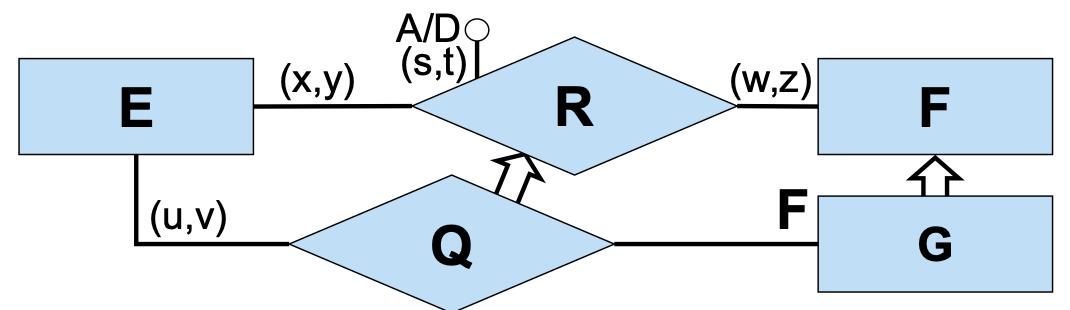
\includegraphics[width=0.4\linewidth]{../images/log1.png}
    %\caption{caption}
    %\label{label}
\end{figure}
\noindent
La nuova entità $R$ è identificata esternamente
mediante le relazioni $RE$ e $RF$, corrispondenti
ai ruoli originari.
Se l'attributo $A$ aveva cardinalità $(s,t)$
e dominio $D$, si introduce inoltre:
\begin{figure}[H]
    \centering  
    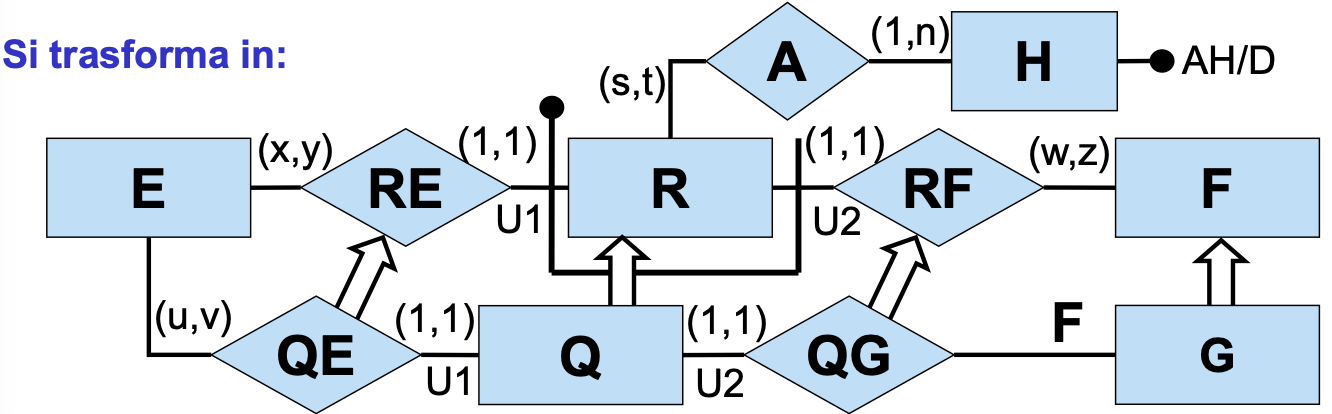
\includegraphics[width=0.5\linewidth]{../images/log2.png}
    %\caption{caption}
    %\label{label}
\end{figure}
\noindent
dove $H$ è identificata da un attributo $AH$
di dominio $D$.

\subsubsection{Attributi multivalore di relazioni:
caso particolare}
È possibile effettuare una trasformazione più semplice
quando sono soddisfatte entrambe le condizioni:

\begin{itemize}
    \item L'attributo multivalore ha cardinalità $(1,n)$.
    \item Tutti i ruoli della relazione $R$ hanno
    cardinalità massima $n$.
\end{itemize}
\noindent
In questo caso non è necessario trasformare $R$
in un'entità.
Si trasforma direttamente l'attributo multivalore
in una nuova entità $H$, collegandola alla relazione
$R$ e aumentandone quindi l'\textbf{arietà}.\\
Ad esempio, una relazione binaria:
\begin{figure}[H]
    \centering  
    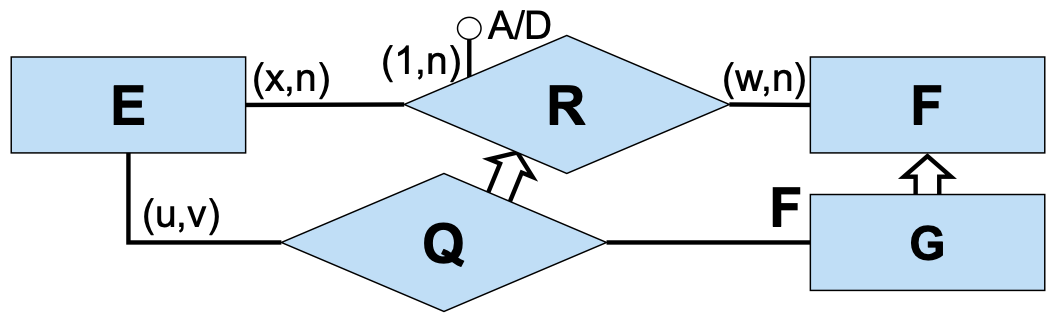
\includegraphics[width=0.4\linewidth]{../images/log3.png}
    %\caption{caption}
    %\label{label}
\end{figure}
\noindent
con attributo multivalore $A$ viene trasformata
in una relazione ternaria:
\begin{figure}[H]
    \centering  
    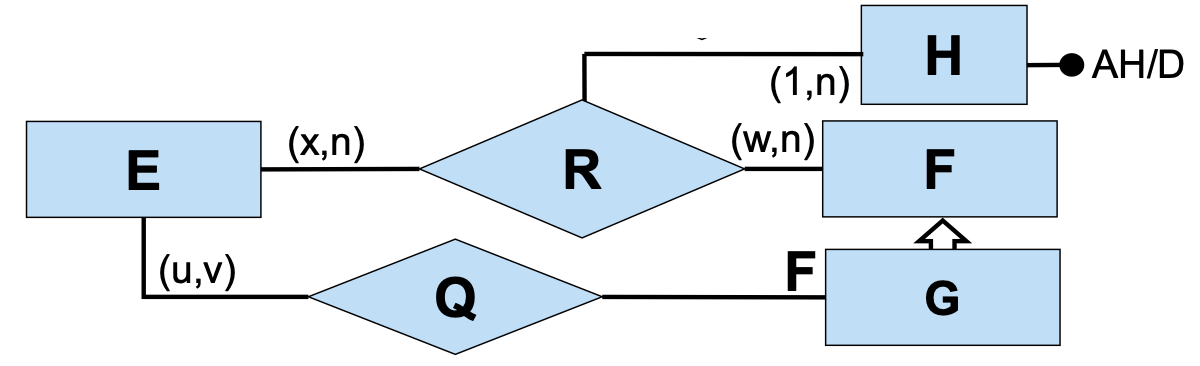
\includegraphics[width=0.5\linewidth]{../images/log4.png}
    %\caption{caption}
    %\label{label}
\end{figure}
\noindent
La nuova entità $H$ rappresenta i valori
dell'attributo $A$ e partecipa a $R$ con
cardinalità $(1,n)$.\\
La cardinalità minima $1$ dell'attributo originario
è fondamentale: ogni istanza originaria di $R$
possiede almeno un valore di $A$ e può quindi
essere rappresentata nella nuova relazione.\medskip\\
\noindent
\textbf{Gestione delle ISA:}
Se originariamente era presente una ISA tra relazioni:
\[
Q \subseteq R
\]
dopo la trasformazione $Q$ rimane binaria, mentre
$R$ diventa ternaria. La ISA non è quindi più
direttamente rappresentabile come prima.\\
Si introduce il seguente vincolo esterno:
\[
\forall(e,f)\in Q,\quad
\exists h\in H : (e,f,h)\in R
\]
Equivalentemente:
\[
Q \subseteq \pi_{E,F}(R)
\]
Ossia, per ogni coppia appartenente a $Q$ deve
esistere almeno una tripla in $R$ contenente
quella coppia.

\subsection{Attività 3: eliminazione degli attributi composti}
Un \textbf{attributo composto} è un attributo
costituito da più attributi componenti.
Poiché gli attributi multivalore sono già stati
eliminati nell'attività precedente, a questo punto
un attributo composto può avere cardinalità
$(1,1)$ oppure $(0,1)$.
La modalità di eliminazione dipende dalla cardinalità.

\subsubsection{Alternativa 1: separazione degli attributi}
Si elimina l'attributo composto e si associano
direttamente i suoi attributi componenti all'entità
o alla relazione originaria.\medskip\\
\noindent
\textcolor{verdeEsempio}{\textbf{Esempio 1. }}
attributo obbligatorio $(1,1)$\\
Si consideri l'entità Persona con l'attributo composto:
\begin{figure}[H]
    \centering  
    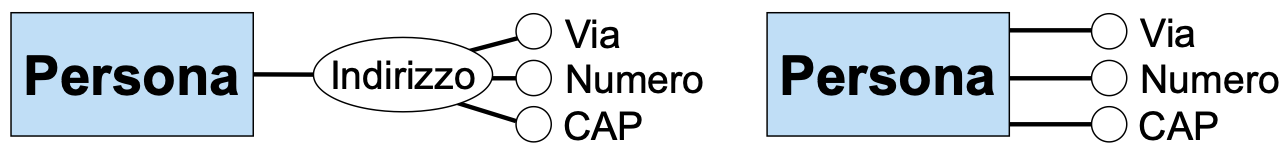
\includegraphics[width=0.5\linewidth]{../images/log5.png}
    %\caption{caption}
    %\label{label}
\end{figure}
\noindent
L'attributo Indirizzo viene eliminato e i suoi
componenti vengono associati direttamente a Persona:
\[
\text{Persona}(\text{Via},\text{Numero},\text{CAP})
\]
In questo esempio tutti e tre gli attributi
mantengono cardinalità $(1,1)$.\medskip\\
\noindent
\textcolor{verdeEsempio}{\textbf{Esempio 2. }}
attributo opzionale $(0,1)$\\
Si consideri l'attributo composto DataMatr
dell'entità Persona, formato da Giorno, Mese e Anno.
Dopo la trasformazione:
\begin{figure}[H]
    \centering  
    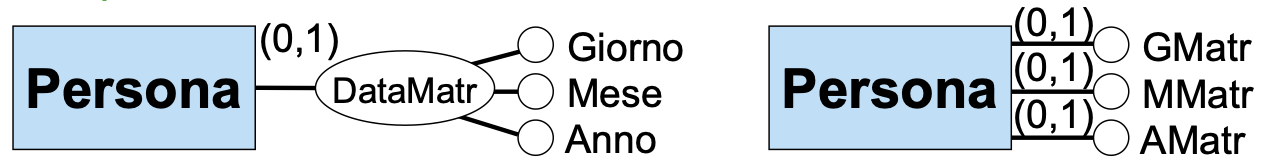
\includegraphics[width=0.5\linewidth]{../images/log6.png}
    %\caption{caption}
    %\label{label}
\end{figure}
\noindent
ciascuno con cardinalità $(0,1)$.\\
Tuttavia, le sole cardinalità non garantiscono
la semantica originaria: una data di matrimonio
non può essere definita soltanto parzialmente.
Occorre quindi introdurre un \textbf{vincolo esterno}
che imponga che i tre attributi siano tutti definiti
oppure tutti non definiti.
\[
\begin{aligned}
&(\text{GMatr definito} \land
  \text{MMatr definito} \land
  \text{AMatr definito})\\
&\lor\\
&(\text{GMatr non definito} \land
  \text{MMatr non definito} \land
  \text{AMatr non definito})
\end{aligned}
\]

\subsubsection{Alternativa 2: introduzione di una nuova entità}
Nel caso di un attributo composto opzionale $(0,1)$,
si può introdurre una nuova entità contenente
gli attributi componenti e sostituire l'attributo
composto con una relazione binaria.\medskip\\
\noindent
\textcolor{verdeEsempio}{\textbf{Esempio. }}
L'attributo composto DataMatr di Persona (esempio precedente) viene
sostituito dall'entità Data:
\begin{figure}[H]
    \centering  
    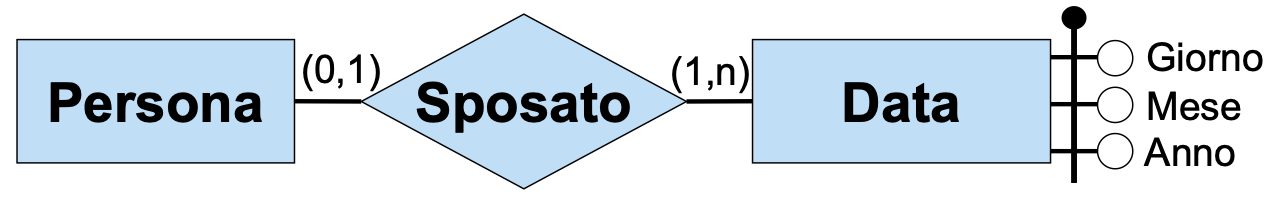
\includegraphics[width=0.5\linewidth]{../images/log7.png}
    %\caption{caption}
    %\label{label}
\end{figure}
\noindent
L'identificatore di Data è costituito dall'insieme
dei tre attributi.
In questo modo:
\begin{itemize}
    \item Una persona può non avere una data di
    matrimonio oppure averne una sola.
    \item Una stessa data può essere associata
    a più persone.
    \item Non è necessario introdurre il vincolo
    esterno dell'alternativa precedente, poiché
    ogni istanza di Data possiede tutti e tre
    gli attributi obbligatori.
\end{itemize}
\noindent
Se l'attributo composto appartiene a una relazione
e si sceglie questa alternativa, occorre prima
trasformare la relazione in un'entità.

\subsection{Attività 4: eliminazione delle ISA tra entità}

Una relazione ISA tra due entità $E$ ed $F$:

\[
E \text{ ISA } F
\]
viene sostituita da una nuova relazione binaria
\textbf{ISA-E-F} tra le due entità, tale che:

\begin{itemize}
    \item $E$ partecipa con cardinalità $(1,1)$,
    poiché ogni istanza dell'entità figlia deve
    corrispondere a un'istanza dell'entità padre.

    \item $F$ partecipa con cardinalità $(0,1)$,
    poiché non tutte le istanze dell'entità padre
    devono appartenere all'entità figlia.
\end{itemize}
\noindent
Agli eventuali identificatori di $E$ viene aggiunto
un \textbf{identificatore esterno}, costituito dalla
partecipazione alla relazione ISA-E-F.\medskip\\
\noindent
\textcolor{verdeEsempio}{\textbf{Esempio. }}
Si consideri la relazione ISA tra Studente e Persona:
\begin{figure}[H]
    \centering
    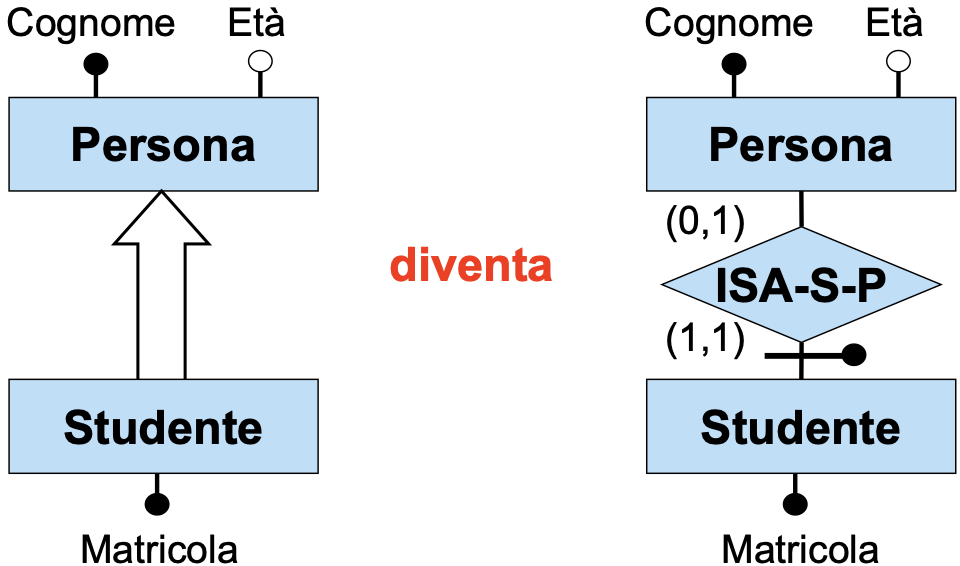
\includegraphics[width=0.50\linewidth]{../images/log8.png}
    %\caption{caption}
    %\label{label}
\end{figure}
\noindent
La ISA viene sostituita dalla relazione ISA-S-P:

\begin{itemize}
    \item Ogni Studente è associato esattamente
    a una Persona.
    \item Ogni Persona è associata al massimo
    a uno Studente.
    \item Studente mantiene il proprio identificatore
    interno Matricola e acquisisce un identificatore
    esterno attraverso ISA-S-P.
\end{itemize}
\noindent
Gli attributi Cognome ed Età rimangono associati
a Persona, mentre Matricola rimane associato
a Studente.

\subsubsection{Eliminazione delle ISA a livello estensionale}

Indichiamo con:

\begin{itemize}
    \item $S_o$: lo schema ER originario.
    \item $S_r$: lo schema ER ottenuto eliminando
    le ISA tra entità.
\end{itemize}
\noindent
Nello schema originario, se $E$ ISA $F$, vale:
\[
\operatorname{istanze}(I,E)
\subseteq
\operatorname{istanze}(I,F)
\]
Ciò significa che uno stesso oggetto può appartenere
contemporaneamente a entrambe le entità.\\
Nello schema ristrutturato, invece, le istanze
delle due entità sono rappresentate mediante
oggetti distinti, collegati dalla relazione ISA-E-F.\medskip\\
\noindent
\textcolor{verdeEsempio}{\textbf{Esempio. }}
Si consideri lo schema originario $S_o$, in cui
$E$ ISA $F$, con $A$ attributo identificatore
di $F$ e $B$ attributo di $E$.

\begin{figure}[H]
    \centering
    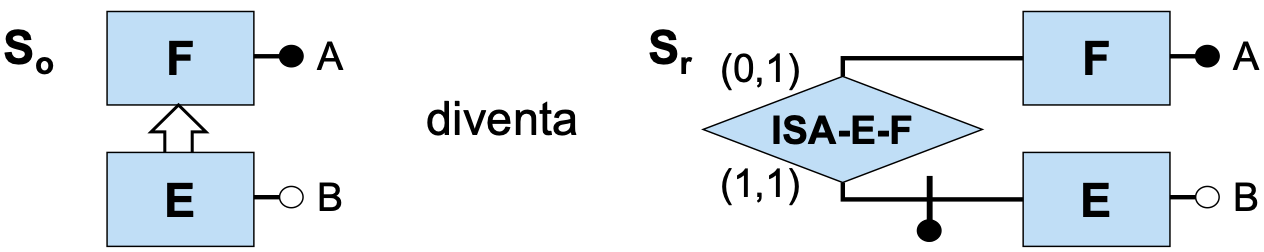
\includegraphics[width=0.60\linewidth]{../images/log9.png}
    %\caption{caption}
    %\label{label}
\end{figure}
\noindent
Nello schema originario, consideriamo l'istanza $I$:

\[
\begin{aligned}
\operatorname{istanze}(I,F)
    &= \{f_1,f_2,f_3\}\\
\operatorname{istanze}(I,E)
    &= \{f_1,f_2\}\\
\operatorname{istanze}(I,A)
    &= \{(f_1,a_1),(f_2,a_2),(f_3,a_3)\}\\
\operatorname{istanze}(I,B)
    &= \{(f_1,b_1),(f_2,b_2)\}
\end{aligned}
\]
Nello schema ristrutturato, si ottiene l'istanza $J$:

\[
\begin{aligned}
\operatorname{istanze}(J,F)
    &= \{f_1,f_2,f_3\}\\
\operatorname{istanze}(J,E)
    &= \{e_1,e_2\}\\
\operatorname{istanze}(J,A)
    &= \{(f_1,a_1),(f_2,a_2),(f_3,a_3)\}\\
\operatorname{istanze}(J,B)
    &= \{(e_1,b_1),(e_2,b_2)\}\\
\operatorname{istanze}(J,\text{ISA-E-F})
    &= \{(e_1,f_1),(e_2,f_2)\}
\end{aligned}
\]
Gli oggetti $f_1$ ed $e_1$ sono distinti nello
schema ristrutturato, ma rappresentano lo stesso
oggetto dello schema originario. Lo stesso vale
per $f_2$ ed $e_2$.\\
\noindent
\textbf{Osservazione:} nello schema risultante
dall'eliminazione di tutte le ISA tra entità,
le entità sono \textbf{disgiunte a coppie},
ossia non hanno più istanze in comune.
L'informazione relativa all'appartenenza di uno
stesso oggetto a più entità viene mantenuta
attraverso le relazioni introdotte.

\subsubsection{Corrispondenza tra istanze}

Esiste una stretta corrispondenza tra le istanze
dello schema originario $S_o$ e quelle dello
schema ristrutturato $S_r$.
Per dimostrare che la trasformazione non comporta
una perdita di informazioni, si introducono
due funzioni totali:

\[
g:\operatorname{istanze}(S_o)
\longrightarrow
\operatorname{istanze}(S_r)
\]
\[
h:\operatorname{istanze}(S_r)
\longrightarrow
\operatorname{istanze}(S_o)
\]
dove:
\begin{itemize}
    \item $g$ trasforma un'istanza dello schema
    originario in un'istanza dello schema ristrutturato.

    \item $h$ ricostruisce un'istanza dello schema
    originario a partire da un'istanza dello
    schema ristrutturato.
\end{itemize}
\noindent
Le due funzioni soddisfano la seguente proprietà:

\[
\boxed{
\forall I_o \in \operatorname{istanze}(S_o),
\qquad h(g(I_o))=I_o
}
\]
\begin{figure}[H]
    \centering
    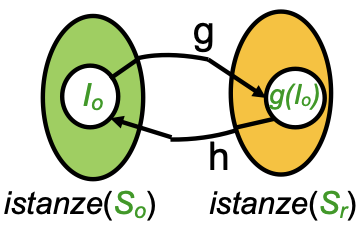
\includegraphics[width=0.25\linewidth]{../images/log10.png}
    %\caption{caption}
    %\label{label}
\end{figure}
\noindent
Ciò significa che, trasformando un'istanza
originaria mediante $g$ e applicando successivamente
$h$, si ottiene esattamente l'istanza di partenza.
La trasformazione permette quindi di
\textbf{preservare la semantica e le informazioni}
dello schema originario.

\subsubsection*{Funzione $g$: dallo schema originario
allo schema ristrutturato}

Sia $I_o$ un'istanza dello schema originario $S_o$.
La funzione $g$ costruisce un'istanza $I_r$ dello
schema ristrutturato $S_r$:

\[
I_r=g(I_o)
\]
La trasformazione avviene nel seguente modo:

\begin{enumerate}
    \item Le istanze dell'entità padre $F$
    rimangono invariate:

    \[
    \operatorname{istanze}(I_r,F)
    =
    \operatorname{istanze}(I_o,F)
    \]

    \item Anche le istanze dell'attributo $A$
    rimangono invariate:

    \[
    \operatorname{istanze}(I_r,A)
    =
    \operatorname{istanze}(I_o,A)
    \]

    \item Per ogni oggetto
    $x\in\operatorname{istanze}(I_o,E)$
    si introduce un nuovo oggetto distinto $g_E(x)$.

    \[
    \operatorname{istanze}(I_r,E)
    =
    \{g_E(x)\mid x\in\operatorname{istanze}(I_o,E)\}
    \]

    \item Si costruisce la relazione ISA-E-F,
    associando ogni nuovo oggetto all'oggetto
    originario:

    \[
    \begin{aligned}
    &\operatorname{istanze}(I_r,\text{ISA-E-F})=\\
    &\quad\{(g_E(x),x)\mid
    x\in\operatorname{istanze}(I_o,E)\}
    \end{aligned}
    \]

    \item Si trasferiscono i valori dell'attributo
    $B$ agli oggetti della nuova entità $E$:

    \[
    \begin{aligned}
    &\operatorname{istanze}(I_r,B)=\\
    &\quad\{(g_E(x),b)\mid
    (x,b)\in\operatorname{istanze}(I_o,B)\}
    \end{aligned}
    \]
\end{enumerate}
\noindent
In sostanza, la funzione $g$ separa gli oggetti
che appartenevano contemporaneamente a $E$ e $F$,
mantenendo la loro corrispondenza attraverso
la relazione ISA-E-F.

\subsubsection*{Funzione $h$: dallo schema ristrutturato
allo schema originario}

Sia $I_r$ un'istanza dello schema ristrutturato $S_r$.
La funzione $h$ ricostruisce un'istanza $I_o$
dello schema originario $S_o$:

\[
I_o=h(I_r)
\]
La ricostruzione avviene nel seguente modo:

\begin{enumerate}
    \item Le istanze dell'entità $F$ e
    dell'attributo $A$ rimangono invariate:

    \[
    \operatorname{istanze}(I_o,F)
    =
    \operatorname{istanze}(I_r,F)
    \]

    \[
    \operatorname{istanze}(I_o,A)
    =
    \operatorname{istanze}(I_r,A)
    \]

    \item Si ricostruiscono le istanze di $E$
    selezionando gli oggetti di $F$ associati
    a un oggetto di $E$ mediante ISA-E-F:

    \[
    \begin{aligned}
    &\operatorname{istanze}(I_o,E)=\\
    &\quad\{x\in\operatorname{istanze}(I_r,F)\mid\\
    &\qquad \exists y\in\operatorname{istanze}(I_r,E):
    (y,x)\in
    \operatorname{istanze}(I_r,\text{ISA-E-F})\}
    \end{aligned}
    \]

    \item Si ricostruiscono i valori dell'attributo
    $B$, associandoli nuovamente agli oggetti
    originari:

    \[
    \begin{aligned}
    &\operatorname{istanze}(I_o,B)=\\
    &\quad\{(x,b)\mid
    x\in\operatorname{istanze}(I_o,E),\\
    &\qquad \exists y\in\operatorname{istanze}(I_r,E):\\
    &\qquad (y,x)\in
    \operatorname{istanze}(I_r,\text{ISA-E-F})\\
    &\qquad \land
    (y,b)\in\operatorname{istanze}(I_r,B)\}
    \end{aligned}
    \]
\end{enumerate}
\noindent
In sostanza, la funzione $h$ ricostruisce
l'appartenenza degli oggetti di $F$ all'entità $E$,
utilizzando le informazioni contenute nella
relazione ISA-E-F.

\subsubsection*{Osservazione sullo schema risultante}

Nonostante nello schema ristrutturato tutte le
entità siano disgiunte a coppie, è possibile
stabilire se due oggetti distinti rappresentano
uno stesso oggetto dello schema originario.
Nell'esempio precedente:

\[
e_1 \longleftrightarrow f_1
\qquad
e_2 \longleftrightarrow f_2
\]
La relazione ISA-E-F conserva l'informazione
relativa all'identità originaria degli oggetti.\\
Le funzioni $g$ e $h$ permettono quindi di
dimostrare che l'eliminazione delle ISA non
comporta una perdita di informazioni:

\[
\boxed{h\circ g=\operatorname{id}}
\]
dove $\operatorname{id}$ è la funzione identità
sull'insieme delle istanze dello schema originario.

\subsubsection{Attributi in comune nell'eliminazione
delle ISA tra entità}

Due entità non disgiunte nello schema originario
possono avere un attributo $A$ in comune.
Dopo l'eliminazione delle ISA, le due entità
diventano disgiunte e i rispettivi attributi $A$
rappresentano due funzioni distinte.\\
Per mantenere la semantica originaria, occorre
garantire che, se due oggetti dello schema
ristrutturato corrispondono allo stesso oggetto
originario, i valori dell'attributo comune
coincidano.\\
Ciò viene garantito mediante un
\textbf{vincolo esterno} sullo schema ristrutturato.\medskip\\
\noindent
\textcolor{verdeEsempio}{\textbf{Esempio. }}
Si considerino le entità Impiegato e Operaio,
entrambe specializzazioni di Persona ed entrambe
dotate dell'attributo Stipendio:

\[
\begin{aligned}
\text{Impiegato}&\text{ ISA Persona}\\
\text{Operaio}&\text{ ISA Persona}
\end{aligned}
\]
\begin{figure}[H]
    \centering
    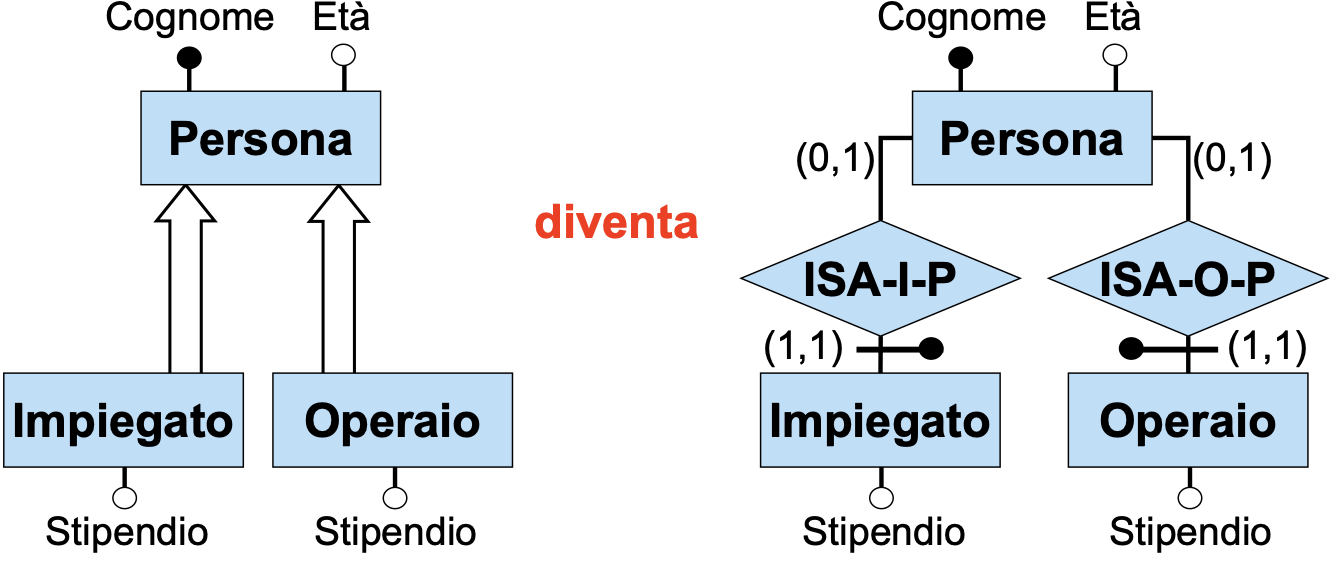
\includegraphics[width=0.7\linewidth]{../images/log11.png}
    %\caption{caption}
    %\label{label}
\end{figure}
\noindent
Nello schema originario una stessa persona può
essere contemporaneamente un Impiegato e un
Operaio.
Poiché Stipendio è un attributo in comune,
esso assume lo stesso valore per tale oggetto.
Dopo l'eliminazione delle ISA si introducono
due relazioni binarie:

\begin{itemize}
    \item ISA-I-P, tra Impiegato e Persona.
    \item ISA-O-P, tra Operaio e Persona.
\end{itemize}
\noindent
Entrambe le relazioni hanno cardinalità $(1,1)$
dal lato dell'entità figlia e $(0,1)$ dal lato
di Persona.
Tuttavia, gli attributi Stipendio di Impiegato
e Operaio rappresentano ora due funzioni distinte
e potrebbero assumere valori differenti.\medskip\\
\noindent
\textbf{Vincolo esterno:} per ogni persona $p$,
se esistono un impiegato $i$ e un operaio $o$
associati entrambi a $p$, allora i due oggetti
devono avere lo stesso stipendio.
Formalmente, utilizzando una notazione semplificata:
\[
\begin{aligned}
\forall p\in\text{Persona},\quad
\forall i\in\text{Impiegato},\quad
\forall o\in\text{Operaio}:\\
\big((i,p)\in\text{ISA-I-P}
\land
(o,p)\in\text{ISA-O-P}\big)\\
\Longrightarrow
\text{Stipendio}(i)=\text{Stipendio}(o)
\end{aligned}
\]
Ad esempio, se una persona è associata sia
a un'istanza di Impiegato sia a un'istanza
di Operaio, non è possibile assegnare
uno stipendio di 1500 euro alla prima
e di 1800 euro alla seconda.
Il vincolo esterno garantisce che l'attributo
comune mantenga la semantica dello schema
originario.
\subsection{Attività 4: Eliminazione delle generalizzazioni tra entità}

Una generalizzazione tra un'entità padre $F$ e le
sottoentità $E_1,E_2,\ldots,E_n$ viene trattata
come un insieme di $n$ relazioni ISA:

\[
E_1 \text{ ISA } F,\ldots,E_n \text{ ISA } F
\]
Si introducono quindi $n$ relazioni binarie:

\[
\text{ISA-}E_1\text{-F},\ldots,
\text{ISA-}E_n\text{-F}
\]
Per ciascuna relazione introdotta:

\begin{itemize}
    \item l'entità figlia $E_i$ partecipa con
    cardinalità $(1,1)$;
    \item l'entità padre $F$ partecipa con
    cardinalità $(0,1)$;
    \item viene aggiunto un identificatore esterno
    all'entità figlia $E_i$, costituito dalla
    partecipazione alla nuova relazione.
\end{itemize}
\noindent
Tuttavia, la semplice eliminazione delle ISA non
è sufficiente a preservare tutte le proprietà
della generalizzazione originaria.
È quindi necessario introdurre opportuni
\textbf{vincoli esterni}, detti
\textbf{vincoli di generalizzazione}.

\subsubsection*{Vincoli di generalizzazione}
\begin{itemize}
    \item \textbf{Generalizzazione non completa:}
    le entità figlie sono disgiunte a coppie,
    ossia per ogni istanza $I$ dello schema:

    \[
    \operatorname{istanze}(I,E_i)
    \cap
    \operatorname{istanze}(I,E_k)
    =\emptyset
    \qquad \forall i\neq k
    \]

    Nello schema ristrutturato tale proprietà
    viene espressa imponendo che ogni istanza
    dell'entità padre $F$ partecipi
    \textbf{al più ad una} delle relazioni
    introdotte.

    \item \textbf{Generalizzazione completa:}
    oltre alla disgiunzione delle entità figlie,
    vale la proprietà:

    \[
    \bigcup_{i=1}^{n}
    \operatorname{istanze}(I,E_i)
    =
    \operatorname{istanze}(I,F)
    \]

    Nello schema ristrutturato si impone quindi
    che ogni istanza dell'entità padre $F$
    partecipi \textbf{esattamente ad una}
    delle relazioni introdotte.
\end{itemize}
\noindent
La differenza consiste quindi nel fatto che,
nel caso non completo, un'istanza dell'entità
padre può non appartenere ad alcuna sottoentità,
mentre nel caso completo deve necessariamente
appartenere a una di esse.\medskip\\
\noindent
\textcolor{verdeEsempio}{\textbf{Esempio. }}
Generalizzazione non completa tra Persona,
Studente e Docente.

\begin{figure}[H]
    \centering
    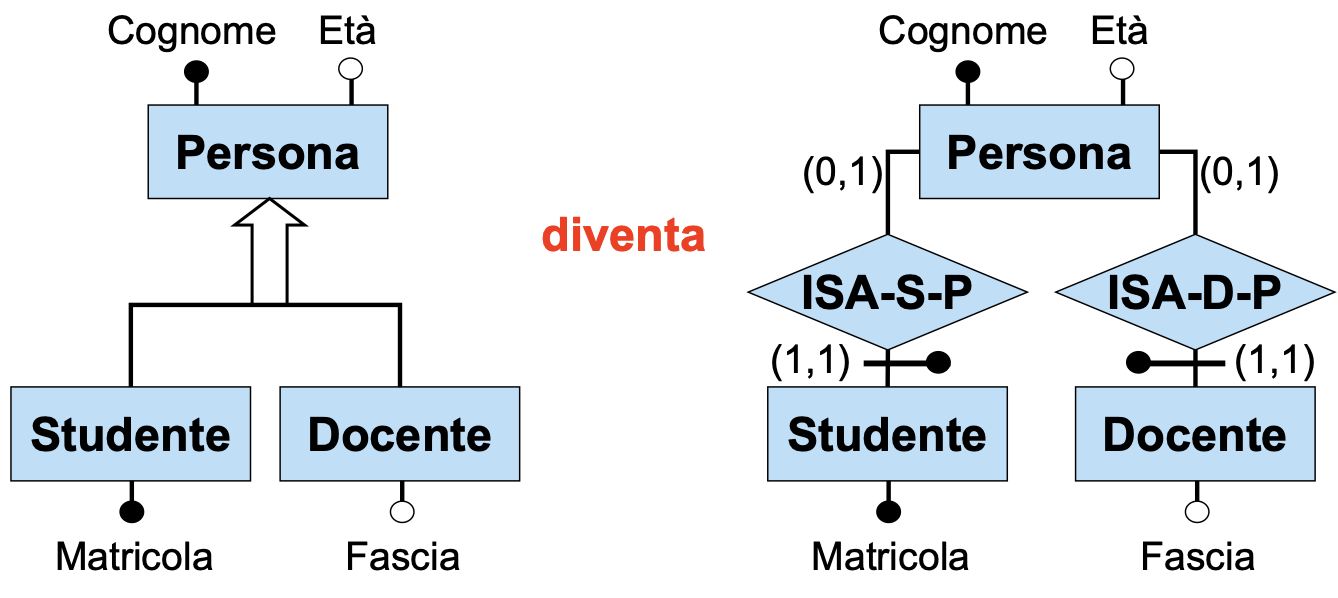
\includegraphics[width=0.7\linewidth]{../images/log12.png}
    %\caption{caption}
    %\label{label}
\end{figure}
\noindent
La generalizzazione viene sostituita dalle
relazioni ISA-S-P e ISA-D-P.
\begin{itemize}
    \item Studente mantiene l'identificatore interno
    Matricola e acquisisce un identificatore
    esterno attraverso ISA-S-P.
    \item Docente acquisisce un identificatore
    esterno attraverso ISA-D-P.
    \item Persona partecipa a entrambe le relazioni
    con cardinalità $(0,1)$.
\end{itemize}
\noindent
\textbf{Vincolo esterno:} nessuna istanza di Persona
può partecipare contemporaneamente a ISA-S-P
e ISA-D-P.\\
Una persona può quindi essere uno studente,
un docente oppure nessuno dei due, ma non può
essere contemporaneamente uno studente e un docente.\medskip\\
\noindent
\textcolor{verdeEsempio}{\textbf{Esempio. }}
Generalizzazione completa tra Persona, Uomo
e Donna, secondo la modellazione proposta
nelle slide.
\begin{figure}[H]
    \centering
    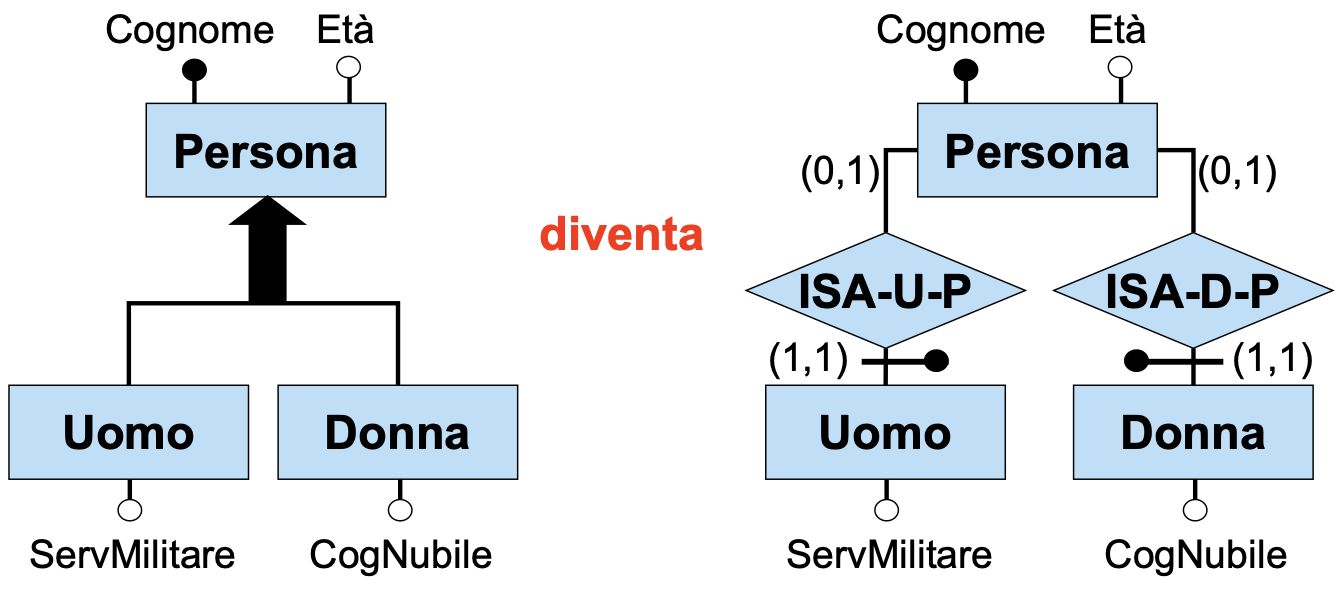
\includegraphics[width=0.9\linewidth]{../images/log13.png}
    %\caption{caption}
    %\label{label}
\end{figure}
\noindent
La generalizzazione viene sostituita dalle
relazioni ISA-U-P e ISA-D-P, mantenendo le
stesse cardinalità utilizzate nel caso precedente.\medskip\\
\noindent
\textbf{Vincolo esterno:} ogni istanza di Persona
deve partecipare a ISA-U-P oppure a ISA-D-P,
ma non a entrambe.\medskip\\
\noindent
\textbf{Osservazione:} le cardinalità delle singole
relazioni introdotte sono identiche sia nel caso
completo sia nel caso non completo. La differenza
tra le due generalizzazioni viene espressa
esclusivamente attraverso i vincoli esterni.


\subsection{Attività 4: Eliminazione delle ISA e delle
generalizzazioni tra relazioni}
Le ISA e le generalizzazioni tra relazioni vengono
eliminate dallo schema e sostituite da opportuni
\textbf{vincoli esterni}.
A differenza dell'eliminazione delle ISA tra
entità, non è necessario introdurre una nuova
relazione per rappresentare direttamente
la ISA tra relazioni.
Si distinguono due casi, a seconda delle entità
che partecipano alle relazioni coinvolte.

\subsubsection*{Relazioni sulle stesse entità}
Se le relazioni coinvolte nella ISA insistono
esattamente sulle stesse entità per tutti i ruoli,
il vincolo esterno può essere espresso direttamente
mediante un'inclusione tra insiemi di istanze.
Data una relazione:
\[
R_1 \text{ ISA } R_2
\]
si elimina la freccia ISA e si introduce il
seguente vincolo esterno:

\[
\boxed{
\operatorname{istanze}(I,R_1)
\subseteq
\operatorname{istanze}(I,R_2)
}
\]
Ogni istanza della relazione figlia deve quindi
essere anche un'istanza della relazione padre.\medskip\\
\noindent
\textcolor{verdeEsempio}{\textbf{Esempio. }}
Si considerino le relazioni Dirige e Lavora,
entrambe definite sulle entità Impiegato e Reparto:
\[
\text{Dirige ISA Lavora}
\]
\begin{figure}[H]
    \centering
    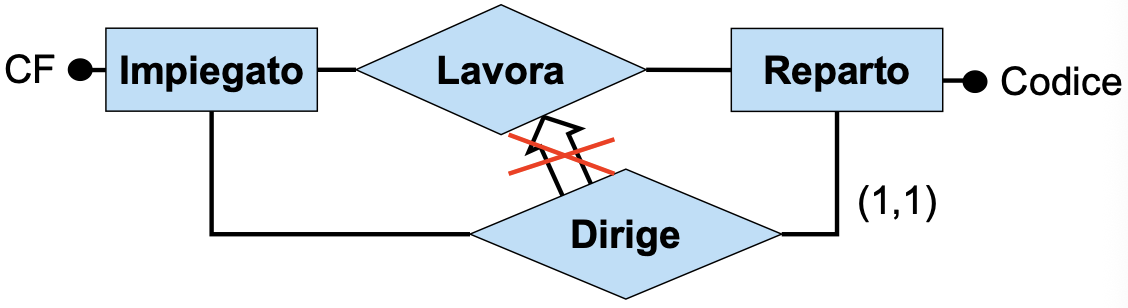
\includegraphics[width=0.55\linewidth]{../images/log141.png}
    %\caption{caption}
    %\label{label}
\end{figure}
\noindent
Si elimina la ISA tra le due relazioni e si
introduce il seguente vincolo esterno:
\[
\operatorname{istanze}(I,\text{Dirige})
\subseteq
\operatorname{istanze}(I,\text{Lavora})
\]
In altre parole, se un impiegato dirige un reparto,
allora deve necessariamente lavorare in quello
stesso reparto.
La cardinalità $(1,1)$ di Reparto rispetto
a Dirige rimane invariata.

\subsubsection*{Relazioni su entità diverse}

Se le relazioni coinvolte nella ISA insistono
su entità diverse in almeno un ruolo, non è
possibile esprimere direttamente il vincolo
mediante un'inclusione tra le rispettive istanze.
Infatti, dopo l'eliminazione delle ISA tra entità,
tutte le entità dello schema ristrutturato sono
\textbf{disgiunte a coppie}.
È quindi necessario utilizzare le relazioni
introdotte durante l'eliminazione delle ISA
tra entità per individuare gli oggetti
corrispondenti.\medskip\\
\noindent
\textcolor{verdeEsempio}{\textbf{Esempio. }}
Si considerino le seguenti ISA:
\[
\begin{aligned}
\text{Direttore}&\text{ ISA Impiegato}\\
\text{Dirige}&\text{ ISA Lavora}
\end{aligned}
\]
La relazione Dirige coinvolge Direttore e Reparto,
mentre Lavora coinvolge Impiegato e Reparto.
\begin{figure}[H]
    \centering
    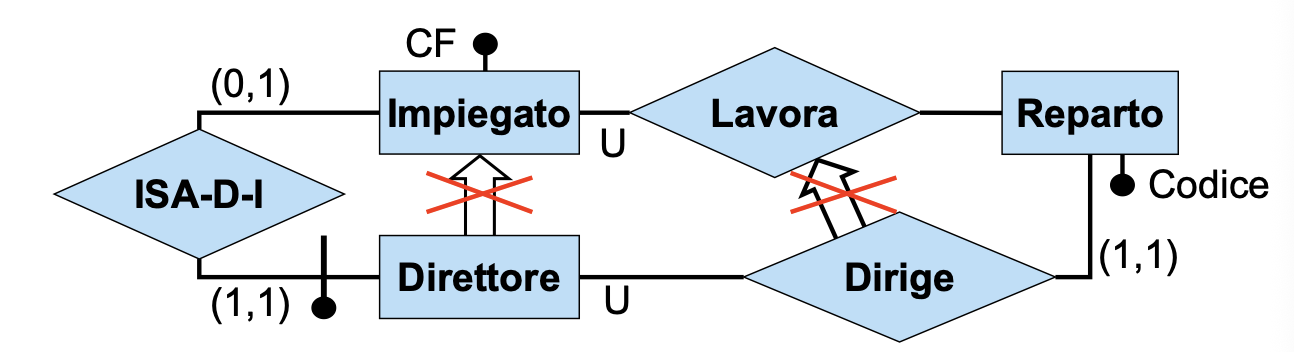
\includegraphics[width=0.9\linewidth]{../images/log15.png}
    %\caption{caption}
    %\label{label}
\end{figure}
\noindent
Eliminando la ISA tra Direttore e Impiegato,
si introduce la relazione ISA-D-I, con cardinalità:

\begin{itemize}
    \item $(1,1)$ dal lato di Direttore;
    \item $(0,1)$ dal lato di Impiegato.
\end{itemize}
\noindent
Nello schema ristrutturato, un direttore $d$
e il corrispondente impiegato $i$ sono due
oggetti distinti, collegati da ISA-D-I.
L'impiegato $i$ associato al direttore $d$
esiste sempre ed è unico, grazie alla cardinalità
$(1,1)$ di Direttore rispetto a ISA-D-I.
In altre parole, se un direttore dirige un reparto,
allora l'impiegato corrispondente a tale direttore
deve lavorare nello stesso reparto.\medskip\\
\noindent
\textbf{Osservazione:} non sarebbe corretto imporre
direttamente:
\[
\operatorname{istanze}(I,\text{Dirige})
\subseteq
\operatorname{istanze}(I,\text{Lavora})
\]
poiché le due relazioni coinvolgono oggetti
appartenenti a entità diverse.
Nel caso delle generalizzazioni tra relazioni,
oltre ai vincoli di inclusione, occorre preservare
anche la disgiunzione delle relazioni figlie
e, nel caso completo, la copertura della
relazione padre, tenendo conto delle
corrispondenze tra gli oggetti.


\subsection{Attività 5: scelta degli identificatori
principali}
La quinta attività della ristrutturazione dello
schema concettuale consiste nella:
\begin{enumerate}
    \item scelta dell'identificatore principale
    di ogni entità;
    \item scelta dell'identificatore principale
    di ogni relazione.
\end{enumerate}
\noindent
Ogni identificatore principale deve essere
necessariamente \textbf{essenziale}.
Un identificatore $K$ di un'entità o relazione
$W$ si dice essenziale se, eliminando un
qualsiasi elemento da $K$, l'insieme risultante
non è più un identificatore di $W$.
Formalmente:
\[
\forall x\in K,\qquad
K\setminus\{x\}
\text{ non è un identificatore di } W
\]
Un identificatore essenziale non contiene quindi
elementi superflui ai fini dell'identificazione.\medskip\\
\noindent
\textcolor{verdeEsempio}{\textbf{Esempio. }}
Si consideri un'entità Studente con gli attributi
Matricola, Nome e Cognome.
Se Matricola identifica univocamente ogni studente,
allora:
\[
K_1=\{\text{Matricola}\}
\]
è un identificatore essenziale, mentre:
\[
K_2=\{\text{Matricola},\text{Nome}\}
\]
non è essenziale, poiché eliminando Nome si
ottiene comunque un identificatore.\medskip\\
\noindent
\textbf{Osservazione:} un identificatore essenziale
non deve necessariamente essere costituito da un
solo elemento. Può essere composto da più elementi,
purché ciascuno di essi sia indispensabile
per l'identificazione.


\subsubsection{Scelta degli identificatori principali
delle entità}

Per ogni entità dello schema ristrutturato
è necessario:

\begin{itemize}
    \item individuare almeno un identificatore;
    \item scegliere, tra gli identificatori
    disponibili, un identificatore principale.
\end{itemize}
\noindent
Se un'entità non possiede alcun identificatore,
è necessario concordare con gli esperti del
dominio l'introduzione di un nuovo attributo,
tipicamente un codice, che possa identificarne
univocamente le istanze.\medskip\\
\noindent
\textbf{Criteri per la scelta dell'identificatore
principale:}

\begin{itemize}
    \item \textbf{Essenzialità:} l'identificatore
    non deve contenere elementi superflui.

    \item \textbf{Semplicità:} si preferiscono
    identificatori costituiti da pochi elementi.

    \item \textbf{Frequenza di utilizzo:} si
    privilegiano gli identificatori utilizzati
    nelle operazioni più frequenti o importanti.

    \item \textbf{Identificazione interna:}
    si preferiscono gli identificatori interni
    rispetto a quelli esterni.

    \item \textbf{Identificazione esterna:}
    tra gli identificatori esterni si privilegiano
    quelli costituiti da relazioni introdotte
    durante l'eliminazione delle ISA.

    \item \textbf{Introduzione di un codice:}
    se nessun identificatore disponibile soddisfa
    adeguatamente i requisiti precedenti, è
    possibile introdurre un nuovo attributo
    avente come unico scopo l'identificazione
    delle istanze dell'entità.
\end{itemize}
\noindent
Se un'entità possiede più identificatori, quello
principale viene indicato nel diagramma dello
schema ristrutturato mediante un
\textbf{cerchio addizionale intorno al pallino
dell'identificatore}.
Gli altri identificatori non vengono eliminati,
poiché continuano a rappresentare vincoli
di identificazione dello schema.
L'identificatore principale sarà utilizzato
nella successiva traduzione verso il modello
relazionale per determinare la chiave primaria.


\subsubsection{Cicli di identificazione esterna
su entità}

Durante la scelta degli identificatori principali
delle entità è necessario evitare la presenza di
\textbf{cicli tra gli identificatori principali
esterni}.
Un ciclo di identificazione esterna si verifica
quando l'identificazione di un'entità dipende,
direttamente o indirettamente, dall'identificazione
dell'entità stessa.
Per individuare tali cicli si costruisce il
\textbf{grafo degli identificatori principali
esterni}.
Il grafo è definito nel seguente modo:

\begin{itemize}
    \item ad ogni entità dello schema corrisponde
    un nodo del grafo;

    \item esiste un arco orientato $E\rightarrow F$
    se e solo se $E$ partecipa a una relazione
    che costituisce, interamente o parzialmente,
    l'identificatore principale esterno di $F$.
\end{itemize}
\noindent
L'arco $E\rightarrow F$ indica quindi che
l'identificazione di $F$ dipende da quella di $E$.
Si ha un ciclo di identificazione esterna quando
il grafo così costruito contiene un ciclo.

\[
E_1\rightarrow E_2\rightarrow\cdots
\rightarrow E_n\rightarrow E_1
\]
La presenza di un ciclo rende problematica
la successiva determinazione delle chiavi,
poiché ciascuna entità del ciclo dipende
dall'identificazione di un'altra entità
del medesimo ciclo.

\subsubsection*{Eliminazione dei cicli di
identificazione esterna}

Per eliminare un ciclo di identificazione
esterna è necessario scegliere, per almeno
una delle entità coinvolte nel ciclo, un
identificatore principale diverso, tale da
spezzare il ciclo.
Se non esistono identificatori alternativi
adeguati, si introduce un nuovo attributo,
tipicamente un codice, da utilizzare come
identificatore principale.\medskip\\
\noindent
\textcolor{verdeEsempio}{\textbf{Esempio. }}
Si consideri il seguente schema con quattro
entità $E_1,E_2,E_3,E_4$.

\begin{figure}[H]
    \centering
    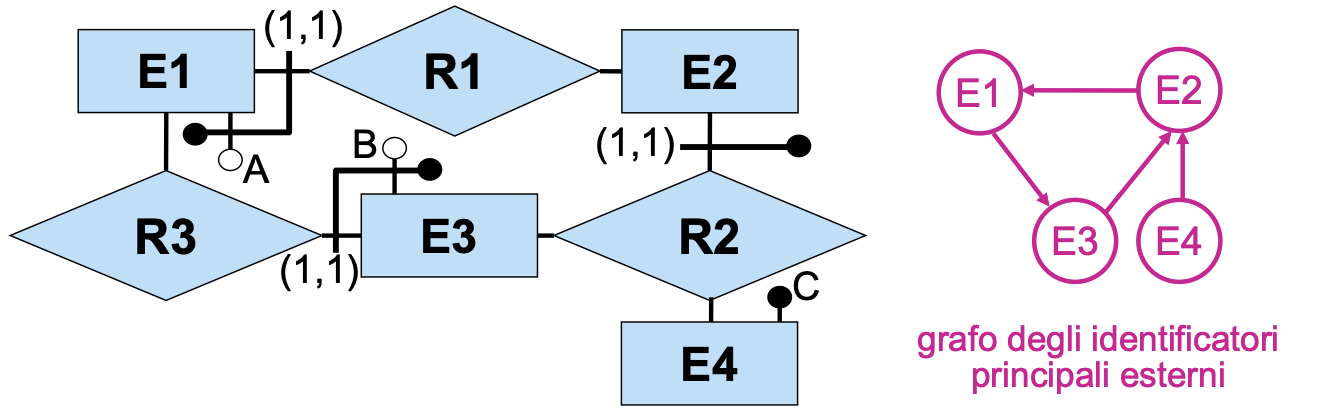
\includegraphics[width=0.9\linewidth]{../images/log16.png}
    %\caption{caption}
    %\label{label}
\end{figure}
\noindent
Gli identificatori principali delle entità
sono costituiti da:

\begin{itemize}
    \item $E_1$: attributo $A$ e partecipazione
    alla relazione $R_1$.
    \item $E_2$: partecipazione alla relazione $R_2$.
    \item $E_3$: attributo $B$ e partecipazione
    alla relazione $R_3$.
    \item $E_4$: attributo $C$.
\end{itemize}
\noindent
Il grafo degli identificatori principali
esterni contiene i seguenti archi:

\[
\begin{aligned}
E_2&\rightarrow E_1\\
E_1&\rightarrow E_3\\
E_3&\rightarrow E_2\\
E_4&\rightarrow E_2
\end{aligned}
\]
Si individua quindi il ciclo:

\[
\boxed{
E_1\rightarrow E_3\rightarrow E_2\rightarrow E_1
}
\]
Infatti:

\begin{itemize}
    \item per identificare $E_1$ è necessario
    identificare $E_2$;
    \item per identificare $E_2$ è necessario
    identificare $E_3$ ed $E_4$;
    \item per identificare $E_3$ è necessario
    identificare $E_1$.
\end{itemize}
\noindent
Si crea quindi una dipendenza circolare
tra gli identificatori principali.
Per spezzare il ciclo si introduce un nuovo
attributo Codice in $E_1$, scegliendolo come
identificatore principale.

\begin{figure}[H]
    \centering
    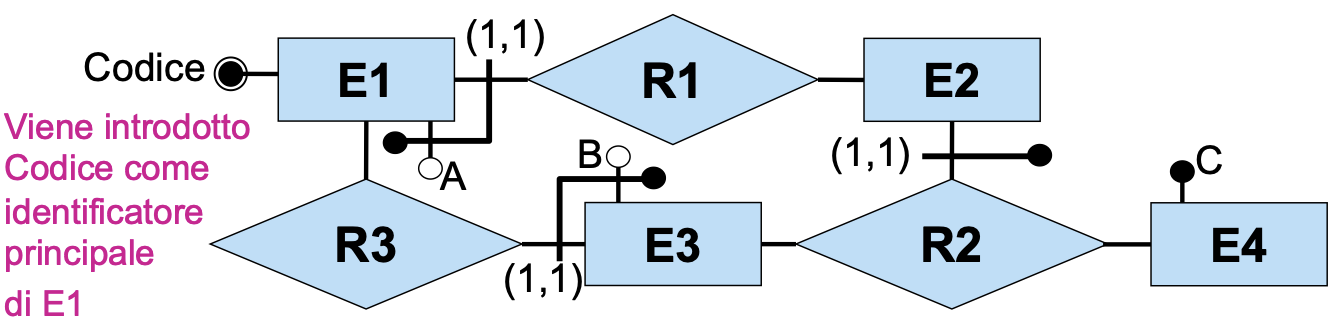
\includegraphics[width=0.65\linewidth]{../images/log17.png}
    %\caption{caption}
    %\label{label}
\end{figure}
\noindent
In questo modo viene eliminato dal grafo
l'arco:

\[
E_2\rightarrow E_1
\]
Il grafo risultante contiene soltanto gli archi:

\[
E_1\rightarrow E_3,\qquad
E_3\rightarrow E_2,\qquad
E_4\rightarrow E_2
\]
e non presenta più cicli.\medskip\\
\noindent
\textbf{Osservazione:} non viene eliminato il
precedente identificatore di $E_1$, costituito
da $A$ e dalla partecipazione a $R_1$.
Esso rimane un identificatore dell'entità,
ma non è più quello principale. Il grafo,
infatti, considera esclusivamente gli
identificatori principali esterni.\medskip\\
\noindent
\textcolor{verdeEsempio}{\textbf{Esempio. }}
Un caso particolare di ciclo di identificazione
esterna si verifica quando due entità si
identificano a vicenda.
Si considerino le entità Rettore e Università,
collegate dalla relazione Di.

\begin{figure}[H]
    \centering
    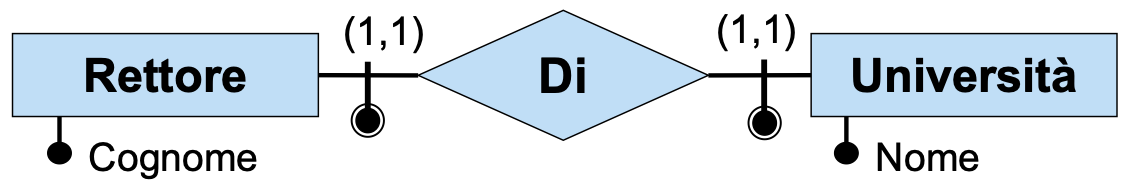
\includegraphics[width=0.45\linewidth]{../images/log18.png}
    %\caption{caption}
    %\label{label}
\end{figure}
\noindent
Entrambe le entità partecipano alla relazione Di
con cardinalità $(1,1)$ e utilizzano tale
partecipazione come identificatore principale.
Pertanto:
\begin{itemize}
    \item Rettore viene identificato attraverso
    Università;
    \item Università viene identificata attraverso
    Rettore.
\end{itemize}
\noindent
Il grafo degli identificatori principali
esterni contiene quindi il ciclo:

\[
\text{Rettore}
\longrightarrow
\text{Università}
\longrightarrow
\text{Rettore}
\]
Per spezzare il ciclo è sufficiente scegliere
come identificatore principale di Università
il suo identificatore interno Nome.

\begin{figure}[H]
    \centering
    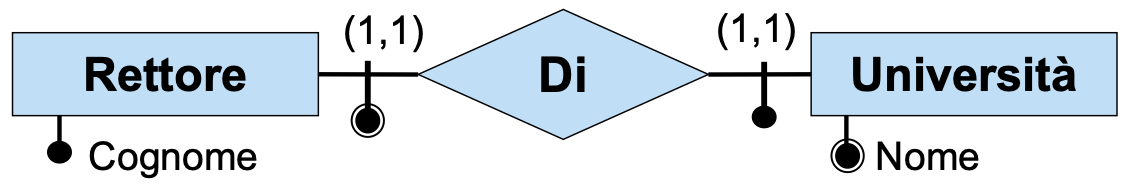
\includegraphics[width=0.45\linewidth]{../images/log19.png}
    %\caption{caption}
    %\label{label}
\end{figure}
\noindent
Rettore continua a essere identificato
principalmente attraverso la relazione Di,
mentre Università viene identificata
principalmente mediante Nome.
Il grafo risultante contiene soltanto l'arco:

\[
\text{Università}\longrightarrow\text{Rettore}
\]
Non è quindi più presente alcun ciclo di
identificazione esterna.
Anche in questo caso non vengono eliminate
né la relazione Di né le cardinalità associate,
ma viene modificata esclusivamente la scelta
dell'identificatore principale di Università.

\subsubsection{Scelta degli identificatori principali delle relazioni}

Per ogni relazione che non partecipa ad un
identificatore principale di entità è necessario
scegliere, tra i suoi identificatori, un
\textbf{identificatore principale}.
I criteri per la scelta sono:

\begin{itemize}
    \item \textbf{Essenzialità:} ogni elemento
    dell'identificatore deve essere indispensabile
    per l'identificazione.

    \item \textbf{Semplicità:} si preferiscono
    identificatori costituiti da pochi elementi.

    \item \textbf{Frequenza di utilizzo:} si
    privilegiano gli identificatori utilizzati
    nelle operazioni più frequenti o importanti.

    \item \textbf{Relazioni derivanti da ISA:}
    si privilegia l'identificatore costituito
    dal ruolo corrispondente all'entità figlia.
\end{itemize}
\noindent
Analogamente a quanto avviene per le entità,
in presenza di più identificatori, quello
principale viene rappresentato mediante un
\textbf{cerchio addizionale intorno al pallino
dell'identificatore}.\medskip\\
\noindent
Nella scelta dell'identificatore principale
di una relazione $R$ si distinguono tre casi:

\begin{enumerate}
    \item \textbf{Relazione che partecipa ad un
    identificatore principale esterno di entità.}

    Se $R$ partecipa all'identificatore principale
    esterno di un'entità $E$, l'identificatore
    principale di $R$ è già determinato attraverso
    l'identificatore di $E$.

    Non è quindi necessario effettuare un'ulteriore
    scelta.

    \item \textbf{Relazione con il solo identificatore
    implicito.}

    Se $R$ non partecipa ad alcun identificatore
    esterno di entità e non possiede identificatori
    espliciti diversi da quello implicito,
    quest'ultimo diventa l'identificatore principale.

    Ricordiamo che l'identificatore implicito
    di una relazione è costituito dall'insieme
    di tutti i suoi ruoli.

    Per una relazione $R$ con ruoli
    $U_1,\ldots,U_n$:

    \[
    K_R=\{U_1,\ldots,U_n\}
    \]

    In questo caso non è obbligatorio rappresentare
    graficamente l'identificatore principale.

    \item \textbf{Relazione con più identificatori.}

    Se $R$ non partecipa ad alcun identificatore
    principale esterno di entità e possiede uno
    o più identificatori espliciti diversi da
    quello implicito, è necessario sceglierne
    uno come principale.

    È possibile scegliere anche l'identificatore
    implicito, purché sia essenziale.

    In questo caso l'identificatore scelto deve
    essere indicato esplicitamente nel diagramma
    dello schema ristrutturato.
\end{enumerate}
\noindent
\textbf{Osservazione:} l'identificatore implicito
deve essere indicato esplicitamente quando viene
scelto come principale in presenza di altri
identificatori, per evitare ambiguità.\medskip\\
\noindent
\textcolor{verdeEsempio}{\textbf{Esempio. }}
Scelta degli identificatori principali delle
relazioni.

\begin{figure}[H]
    \centering
    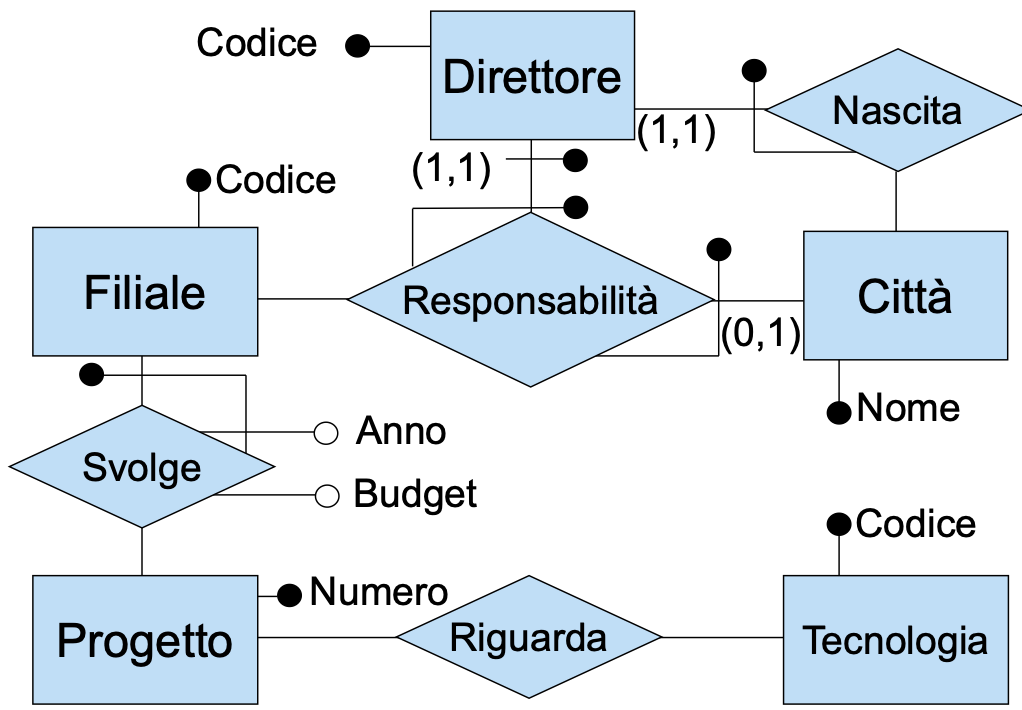
\includegraphics[width=0.50\linewidth]{../images/log20.png}
    %\caption{caption}
    %\label{label}
\end{figure}
\noindent
Si supponga che le operazioni più frequenti
utilizzino:

\begin{itemize}
    \item il Codice per accedere ai direttori;
    \item la Città per accedere alle informazioni
    sulla Responsabilità;
    \item la combinazione di Filiale e Progetto
    per accedere alle informazioni sullo
    svolgimento dei progetti.
\end{itemize}
\noindent
Sulla base di queste informazioni vengono
effettuate le seguenti scelte.

\begin{figure}[H]
    \centering
    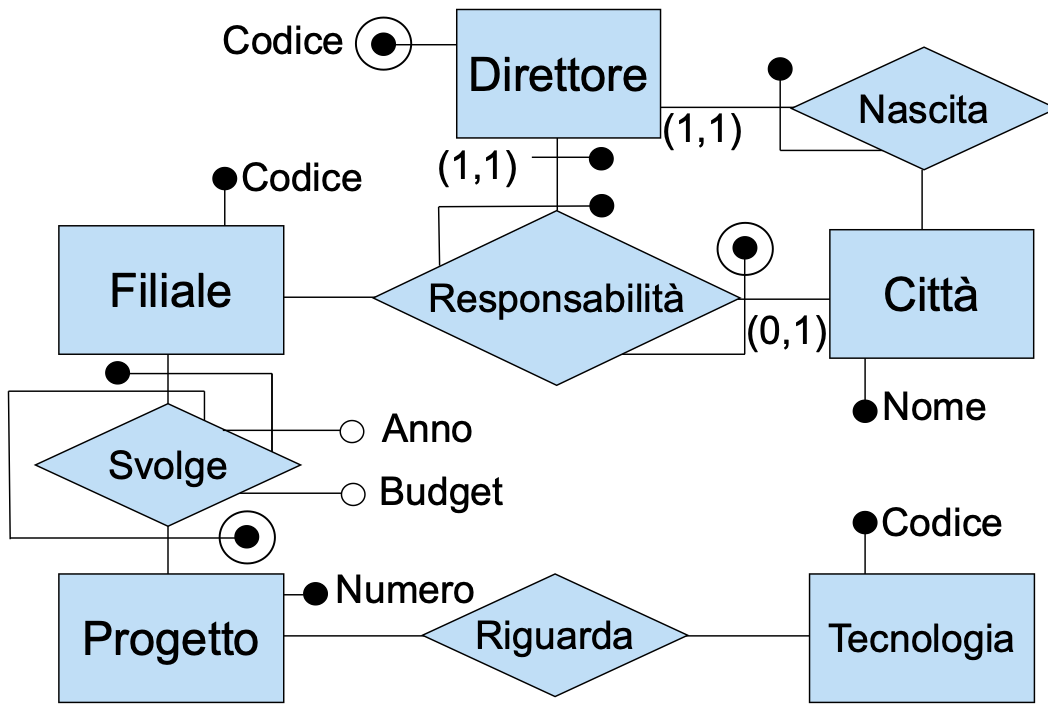
\includegraphics[width=0.50\linewidth]{../images/log21.png}
    %\caption{caption}
    %\label{label}
\end{figure}

\begin{itemize}
    \item \textbf{Direttore:} viene scelto Codice
    come identificatore principale, poiché
    utilizzato nelle operazioni più frequenti.

    \item \textbf{Responsabilità:} viene scelto
    il ruolo corrispondente a Città come
    identificatore principale.

    Infatti, la cardinalità $(0,1)$ di Città
    garantisce che una città partecipi al più
    ad un'istanza di Responsabilità.

    \item \textbf{Svolge:} viene scelto
    l'identificatore implicito:

    \[
    K_{\text{Svolge}}=
    \{\text{Filiale},\text{Progetto}\}
    \]

    La relazione possiede anche l'identificatore
    esplicito:

    \[
    \{\text{Anno},\text{Filiale}\}
    \]

    Poiché le operazioni utilizzano principalmente
    la filiale e il numero del progetto, si
    preferisce l'identificatore implicito.

    È necessario rappresentarlo esplicitamente
    nel diagramma, altrimenti l'identificatore
    $(\text{Anno},\text{Filiale})$ verrebbe
    interpretato come principale.

    \item \textbf{Riguarda:} viene scelto
    l'identificatore implicito:

    \[
    K_{\text{Riguarda}}=
    \{\text{Progetto},\text{Tecnologia}\}
    \]

    Non essendoci altri identificatori espliciti,
    non è necessario rappresentarlo nel diagramma.

    \item \textbf{Nascita:} viene identificata
    attraverso il ruolo Direttore, poiché ogni
    direttore partecipa esattamente ad un'istanza
    della relazione Nascita.
\end{itemize}
\noindent
La scelta dell'identificatore principale non
comporta l'eliminazione degli altri identificatori,
che continuano a rappresentare vincoli dello
schema.


\subsection{Attività 6: specifica degli ulteriori
vincoli esterni}

L'ultima attività della ristrutturazione consiste
nella specifica di tutti i vincoli che non sono
rappresentati direttamente nello schema
ristrutturato.
È necessario:

\begin{itemize}
    \item riformulare tutti i vincoli esterni
    dello schema originario utilizzando le
    entità, le relazioni e gli attributi dello
    schema ristrutturato;

    \item mettere in evidenza eventuali
    \textbf{vincoli impliciti}, ossia vincoli
    che derivano da altri vincoli già presenti;

    \item aggiungere i nuovi vincoli esterni
    derivanti dalle attività di ristrutturazione.
\end{itemize}

\noindent
I principali vincoli derivanti dalla
ristrutturazione sono:

\begin{itemize}
    \item \textbf{Vincoli sugli attributi
    composti opzionali:} necessari per
    preservare la semantica dell'attributo
    composto dopo la sua eliminazione.

    \item \textbf{Vincoli sugli attributi
    comuni:} necessari quando due entità,
    precedentemente in ISA con una stessa
    entità padre, possiedono uno stesso
    attributo.

    \item \textbf{Vincoli di generalizzazione:}
    necessari per preservare le proprietà
    di disgiunzione e completezza dopo
    l'eliminazione delle generalizzazioni.

    \item \textbf{Vincoli sugli identificatori
    non principali:} necessari qualora tali
    identificatori non siano più rappresentati
    direttamente nello schema.
\end{itemize}
\noindent
\textcolor{verdeEsempio}{\textbf{Esempio. }}
Si consideri una relazione binaria $R$ tra
due entità $E$ ed $F$, con cardinalità
$(1,1)$ dal lato di $E$ e $(0,1)$ dal lato
di $F$.
Ogni istanza di $E$ è associata esattamente
ad un'istanza di $F$ e ogni istanza di $F$
è associata al più ad un'istanza di $E$.
Pertanto, la partecipazione alla relazione
$R$ costituisce un identificatore esterno
di $E$, anche se questo non era stato
indicato esplicitamente nello schema
originario.
Tale vincolo di identificazione deve essere
messo in evidenza durante la ristrutturazione.


\subsection{Riassunto delle attività di ristrutturazione}

La ristrutturazione dello schema concettuale
ER si articola nelle seguenti attività:

\begin{enumerate}
    \setcounter{enumi}{-1}

    \item \textbf{Preparazione iniziale dello
    schema ER.}

    \item \textbf{Analisi delle ridondanze.}

    Si valuta se mantenere o eliminare le
    informazioni ridondanti, tenendo conto
    dell'efficienza delle operazioni.

    \item \textbf{Eliminazione degli attributi
    multivalore.}

    Gli attributi multivalore vengono sostituiti
    mediante opportune entità e relazioni.

    \item \textbf{Eliminazione degli attributi
    composti.}

    Gli attributi composti vengono sostituiti
    dai rispettivi attributi componenti.

    Eventuali cardinalità $(0,1)$ vengono
    rappresentate mediante opportuni vincoli
    esterni.

    \item \textbf{Eliminazione delle ISA e
    delle generalizzazioni.}

    \begin{itemize}
        \item Le ISA tra entità vengono sostituite
        da relazioni binarie.

        \item Le ISA tra relazioni vengono
        sostituite da vincoli esterni.

        \item Si introducono vincoli sugli
        attributi comuni delle entità figlie.

        \item Si introducono vincoli di
        disgiunzione e completezza.

        \item Tutte le entità dello schema
        ristrutturato diventano disgiunte.
    \end{itemize}

    \item \textbf{Scelta degli identificatori
    principali di entità e relazioni.}

    \begin{itemize}
        \item Ogni entità deve possedere almeno
        un identificatore.

        \item Se necessario, si introducono
        nuovi attributi di tipo codice.

        \item Si scelgono identificatori
        principali essenziali.

        \item Si eliminano eventuali cicli
        di identificazione principale esterna.
    \end{itemize}

    \item \textbf{Specifica degli ulteriori
    vincoli esterni.}

    \begin{itemize}
        \item Si aggiungono i vincoli derivanti
        dalla ristrutturazione.

        \item Si riformulano i vincoli esterni
        dello schema originario.
    \end{itemize}
\end{enumerate}
\noindent
Al termine della ristrutturazione si ottiene
uno schema ER adatto alla successiva traduzione
nel modello relazionale, preservando la semantica
dello schema concettuale originario.\medskip\\
\noindent
\textcolor{verdeEsempio}{\textbf{Esercizio 3. }}
Ristrutturazione di uno schema relativo ai voli
e alle compagnie aeree.

\begin{figure}[H]
    \centering
    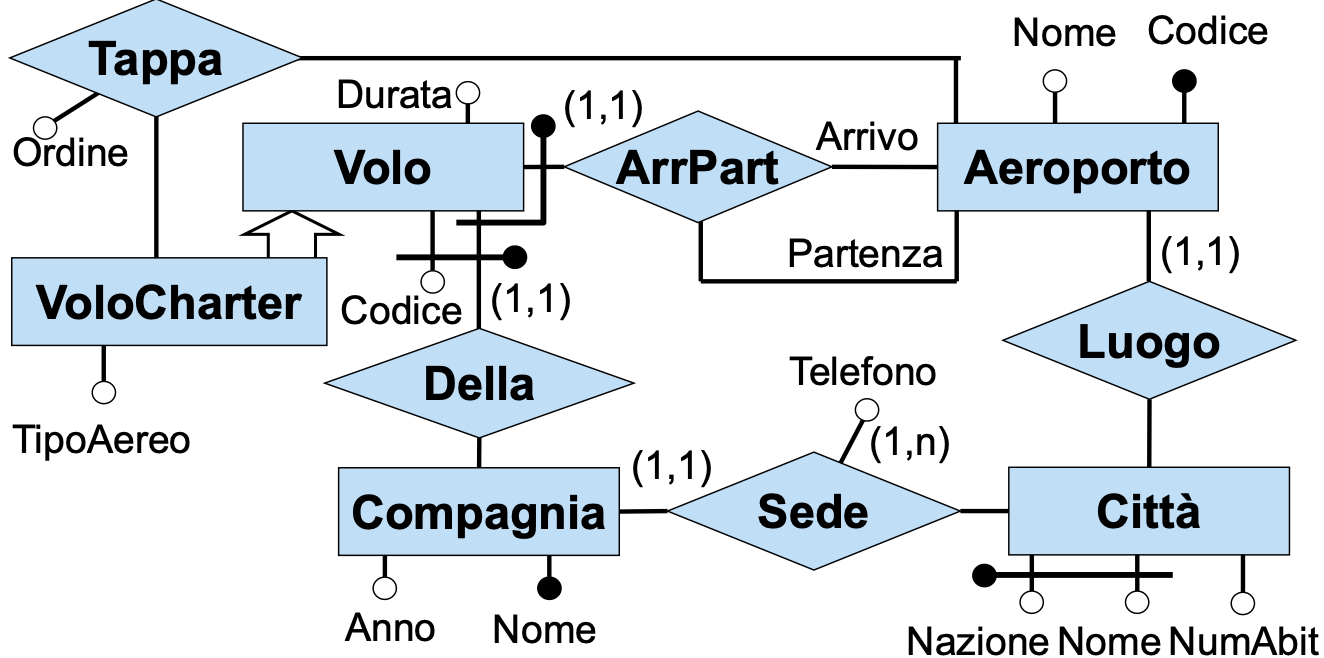
\includegraphics[width=0.5\linewidth]{../images/log22.png}
    %\caption{caption}
    %\label{label}
\end{figure}
\noindent
Lo schema originario presenta una relazione
ISA tra VoloCharter e Volo, un attributo
multivalore Telefono associato alla relazione
Sede e diversi identificatori esterni.
Sono inoltre presenti due vincoli esterni:

\begin{enumerate}
    \item Per ogni volo charter con $n$ tappe,
    i valori dell'attributo Ordine devono
    corrispondere ai numeri interi da $1$ a $n$.

    Indicando con $o_1,\ldots,o_n$ i valori
    dell'attributo Ordine:

    \[
    \{o_1,\ldots,o_n\}=\{1,\ldots,n\}
    \]

    \item Ogni numero di telefono appartiene
    ad una sola sede.
\end{enumerate}
\noindent
\textbf{Soluzione:}

\begin{figure}[H]
    \centering
    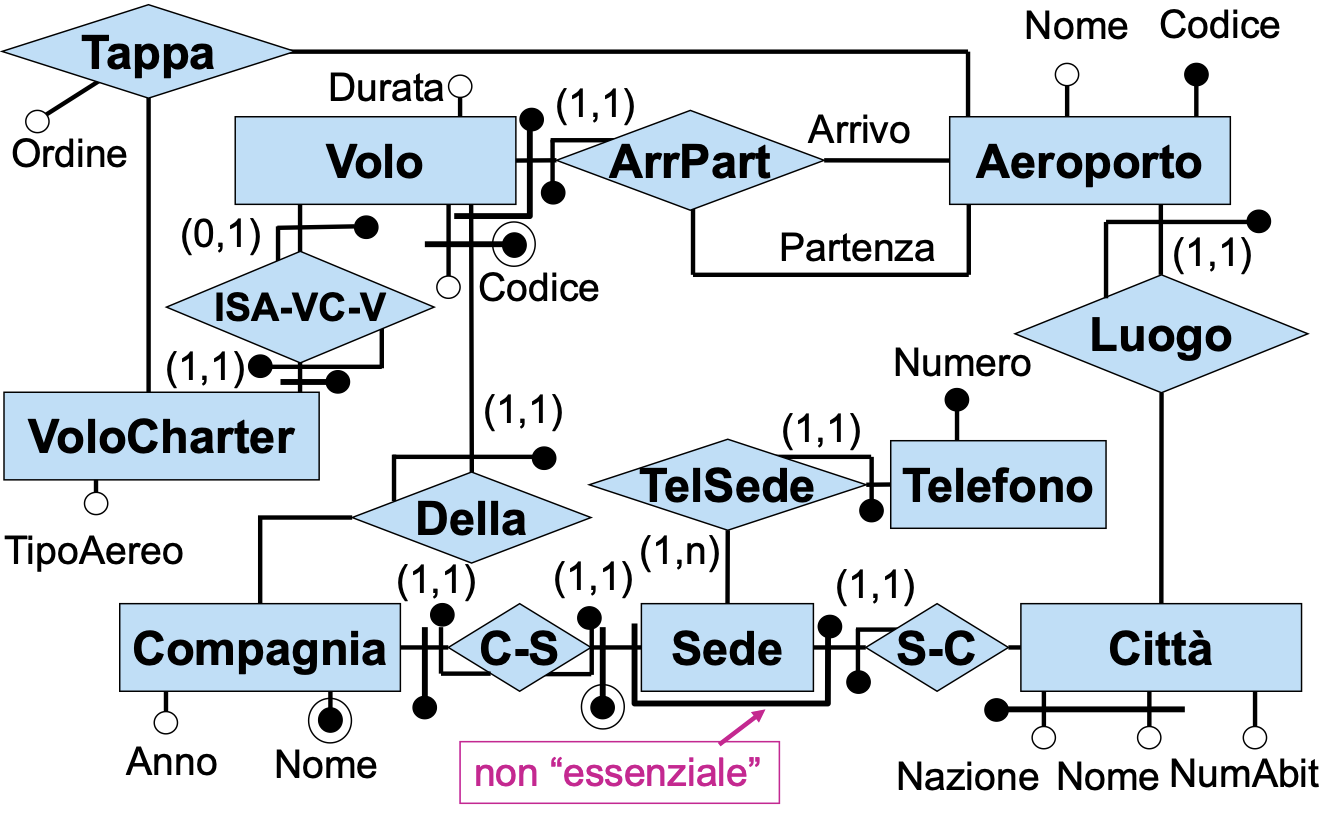
\includegraphics[width=0.60\linewidth]{../images/log23.png}
    %\caption{caption}
    %\label{label}
\end{figure}
\noindent
Le principali trasformazioni effettuate sono:

\begin{enumerate}
    \item \textbf{Eliminazione dell'attributo
    multivalore Telefono.}

    Poiché Telefono è un attributo multivalore
    della relazione Sede, è necessario
    trasformare quest'ultima in un'entità.

    Vengono introdotte le entità Sede e Telefono,
    insieme alle relazioni:

    \begin{itemize}
        \item C-S, tra Compagnia e Sede;
        \item S-C, tra Sede e Città;
        \item TelSede, tra Sede e Telefono.
    \end{itemize}

    La relazione C-S presenta cardinalità
    $(1,1)$ da entrambi i lati, poiché ogni
    compagnia possiede esattamente una sede
    e ogni sede corrisponde ad una compagnia.
    La relazione S-C presenta cardinalità
    $(1,1)$ dal lato di Sede, poiché ogni
    sede è situata in una sola città.
    La relazione TelSede presenta cardinalità:

    \[
    \begin{aligned}
    \text{Sede}&:\ (1,n)\\
    \text{Telefono}&:\ (1,1)
    \end{aligned}
    \]
    Ogni sede possiede almeno un numero
    di telefono, mentre ogni numero appartiene
    esattamente ad una sede.
    Telefono viene identificato attraverso
    l'attributo Numero.
    \item \textbf{Eliminazione della ISA tra
    VoloCharter e Volo.}
    La relazione:
    \[
    \text{VoloCharter ISA Volo}
    \]
    viene sostituita dalla relazione binaria
    ISA-VC-V, con cardinalità:

    \[
    \begin{aligned}
    \text{VoloCharter}&:\ (1,1)\\
    \text{Volo}&:\ (0,1)
    \end{aligned}
    \]
    VoloCharter acquisisce un identificatore
    esterno attraverso ISA-VC-V.
    Ogni volo charter è associato esattamente
    ad un volo, mentre non tutti i voli sono
    necessariamente voli charter.

    \item \textbf{Esplicitazione degli
    identificatori impliciti.}

    Vengono messi in evidenza gli identificatori
    delle relazioni che derivano dalle
    cardinalità massime uguali a $1$.
    Ad esempio, ArrPart è identificata dal
    ruolo Volo, poiché ogni volo partecipa
    esattamente ad un'istanza di ArrPart.
    Analogamente, Luogo è identificata dal
    ruolo Aeroporto e Della dal ruolo Volo.

    \item \textbf{Scelta degli identificatori
    principali.}

    Volo possiede due identificatori esterni
    composti:
    \begin{itemize}
        \item Codice e partecipazione ad ArrPart;
        \item Codice e partecipazione a Della.
    \end{itemize}

    Nella soluzione viene scelto come
    identificatore principale quello costituito
    da Codice e dalla partecipazione a Della.
    Compagnia viene identificata principalmente
    attraverso Nome.
    Sede può essere identificata attraverso
    la sola partecipazione a C-S, poiché
    ogni compagnia è associata ad una sola sede.
    L'identificatore costituito congiuntamente
    dalle partecipazioni a C-S e S-C non è
    essenziale.
    Infatti, eliminando S-C, la partecipazione
    a C-S è già sufficiente per identificare
    univocamente una sede.
\end{enumerate}
\noindent
\textbf{Vincoli esterni dopo la ristrutturazione:}
Il vincolo relativo all'attributo Ordine
della relazione Tappa rimane un vincolo
esterno, poiché non può essere espresso
mediante le sole cardinalità dello schema.
Il vincolo secondo cui ogni numero di
telefono appartiene ad una sola sede
diventa invece un \textbf{vincolo interno
allo schema}, grazie all'identificatore
Numero di Telefono e alla cardinalità
$(1,1)$ rispetto a TelSede.\medskip\\
\noindent
\textbf{Osservazione:} la ristrutturazione può
trasformare alcuni vincoli esterni dello
schema originario in vincoli direttamente
rappresentabili nel diagramma ER.\medskip\\
\noindent
\textcolor{verdeEsempio}{\textbf{Esercizio 4. }}
Ristrutturazione di uno schema relativo alle
officine e alle riparazioni dei veicoli.

\begin{figure}[H]
    \centering
    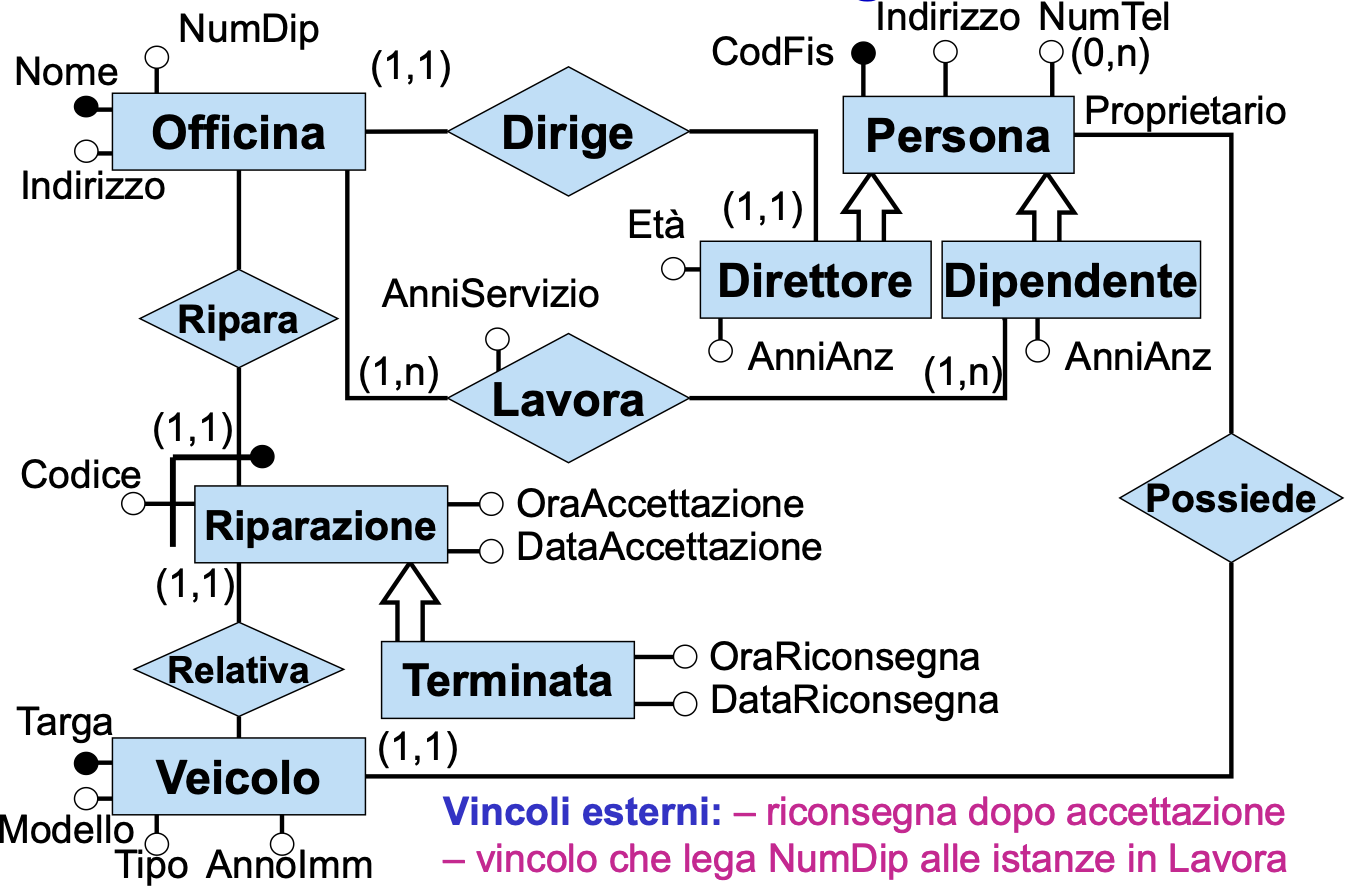
\includegraphics[width=0.5\linewidth]{../images/log24.png}
    %\caption{caption}
    %\label{label}
\end{figure}
\noindent
Lo schema originario presenta:

\begin{itemize}
    \item l'attributo multivalore NumTel
    dell'entità Persona;

    \item le ISA di Direttore e Dipendente
    rispetto a Persona;

    \item la ISA di Terminata rispetto a
    Riparazione;

    \item l'attributo AnniAnz presente sia
    in Direttore sia in Dipendente;

    \item l'attributo ridondante NumDip
    dell'entità Officina.
\end{itemize}
\noindent
Sono inoltre presenti due vincoli esterni:

\begin{itemize}
    \item la riconsegna di un veicolo deve
    avvenire dopo la sua accettazione;

    \item il valore di NumDip deve essere
    coerente con le istanze della relazione
    Lavora.
\end{itemize}
\noindent
\textbf{Soluzione:}

\begin{figure}[H]
    \centering
    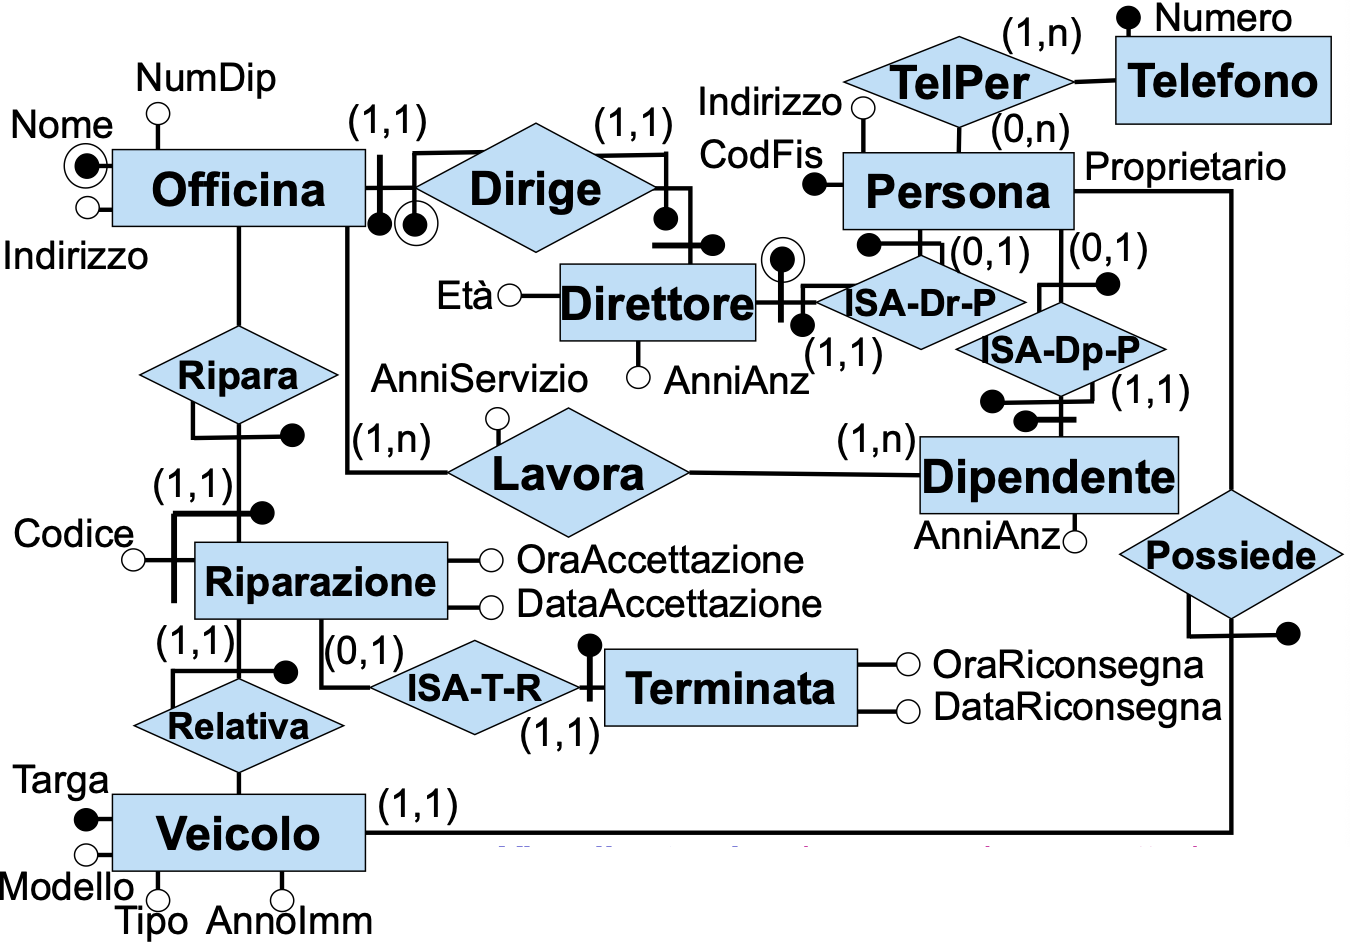
\includegraphics[width=0.60\linewidth]{../images/log25.png}
    %\caption{caption}
    %\label{label}
\end{figure}
\noindent
Le principali trasformazioni effettuate sono:

\begin{enumerate}
    \item \textbf{Analisi delle ridondanze.}

    L'attributo NumDip rappresenta il numero
    di dipendenti che lavorano in un'officina
    ed è ricavabile dalla relazione Lavora.

    Nella soluzione si decide di mantenere
    tale ridondanza.

    È quindi necessario mantenere il vincolo:

    \[
    \forall o\in\text{Officina},\qquad
    \text{NumDip}(o)=
    |\{d\mid(o,d)\in\text{Lavora}\}|
    \]

    Tale vincolo garantisce la coerenza
    tra il valore memorizzato e le istanze
    della relazione Lavora.

    \item \textbf{Eliminazione dell'attributo
    multivalore NumTel.}

    L'attributo NumTel di Persona viene
    sostituito dall'entità Telefono, identificata
    mediante l'attributo Numero, e dalla
    relazione TelPer.
    Le cardinalità sono:

    \[
    \begin{aligned}
    \text{Persona}&:\ (0,n)\\
    \text{Telefono}&:\ (1,n)
    \end{aligned}
    \]
    Una persona può non possedere alcun
    numero di telefono oppure possederne
    più di uno.
    Uno stesso numero di telefono può
    essere associato a più persone.

    \item \textbf{Eliminazione delle ISA
    tra Direttore, Dipendente e Persona.}

    Le due ISA vengono sostituite dalle
    relazioni binarie:

    \[
    \begin{aligned}
    &\text{ISA-Dr-P}\\
    &\text{ISA-Dp-P}
    \end{aligned}
    \]
    Entrambe presentano cardinalità $(1,1)$
    dal lato dell'entità figlia e $(0,1)$
    dal lato di Persona.
    Direttore e Dipendente acquisiscono
    un identificatore esterno attraverso
    le rispettive relazioni ISA.
    \textbf{Attenzione:} nello schema originario
    sono presenti due ISA distinte e non
    una generalizzazione.
    Pertanto, una stessa persona può essere
    contemporaneamente un direttore e un
    dipendente.
    Non deve essere introdotto alcun vincolo
    di disgiunzione tra le due specializzazioni.

    \item \textbf{Eliminazione della ISA
    tra Terminata e Riparazione.}

    La ISA viene sostituita dalla relazione
    ISA-T-R, con cardinalità:

    \[
    \begin{aligned}
    \text{Terminata}&:\ (1,1)\\
    \text{Riparazione}&:\ (0,1)
    \end{aligned}
    \]
    Ogni riparazione terminata corrisponde
    esattamente ad una riparazione, mentre
    una riparazione può non essere ancora
    terminata.
    Terminata viene identificata esternamente
    attraverso ISA-T-R.

    \item \textbf{Esplicitazione degli
    identificatori impliciti.}

    La relazione Dirige presenta cardinalità
    $(1,1)$ da entrambi i lati.
    Di conseguenza, Officina e Direttore
    possono identificarsi reciprocamente
    attraverso tale relazione.
    Si rendono inoltre espliciti gli
    identificatori delle relazioni Ripara,
    Relativa e Possiede, derivanti dalle
    rispettive cardinalità $(1,1)$.

    \item \textbf{Scelta degli identificatori
    principali.}

    Officina possiede sia l'identificatore
    interno Nome sia un identificatore
    esterno attraverso Dirige.
    Viene scelto Nome come identificatore
    principale.
    Direttore viene identificato principalmente
    attraverso ISA-Dr-P, privilegiando
    l'identificatore esterno derivante
    dall'eliminazione della ISA.
    Per la relazione Dirige viene scelto
    come identificatore principale il ruolo
    Officina.
    Riparazione mantiene l'identificatore
    composto costituito da Codice e dalla
    partecipazione alla relazione Ripara.
    In questo modo non vengono introdotti
    cicli tra gli identificatori principali
    esterni.
\end{enumerate}

\noindent
\textbf{Vincoli esterni dopo la ristrutturazione:}

\begin{itemize}
    \item \textbf{Vincolo temporale:}

    per ogni riparazione terminata, la data
    e l'ora di riconsegna devono essere
    successive alla data e all'ora di
    accettazione della corrispondente
    riparazione.

    \item \textbf{Vincolo di ridondanza:}

    il valore di NumDip deve coincidere
    con il numero di dipendenti associati
    all'officina attraverso Lavora.

    \item \textbf{Vincolo sull'attributo
    comune AnniAnz:}

    se una persona è contemporaneamente
    un direttore e un dipendente, i valori
    dell'attributo AnniAnz nelle due entità
    devono coincidere.
\end{itemize}

\section{Traduzione diretta nel modello relazionale}
